\section{Implémentation}

L’implémentation du logiciel a été réalisée par étapes, en suivant les \textit{job stories} décrites en \autoref{sec:annexes_b}, ainsi que les tâches planifiées dans le diagramme de Gantt présenté en \autoref{fig:gantt_prototype_phases_detailed} (\autoref{sec:méthodologie}).

La \autoref{fig:structure_interactions} illustre l’architecture logicielle globale ainsi que les interactions entre les deux projets (client et robot).

\begin{figure}[H]
    \centering
    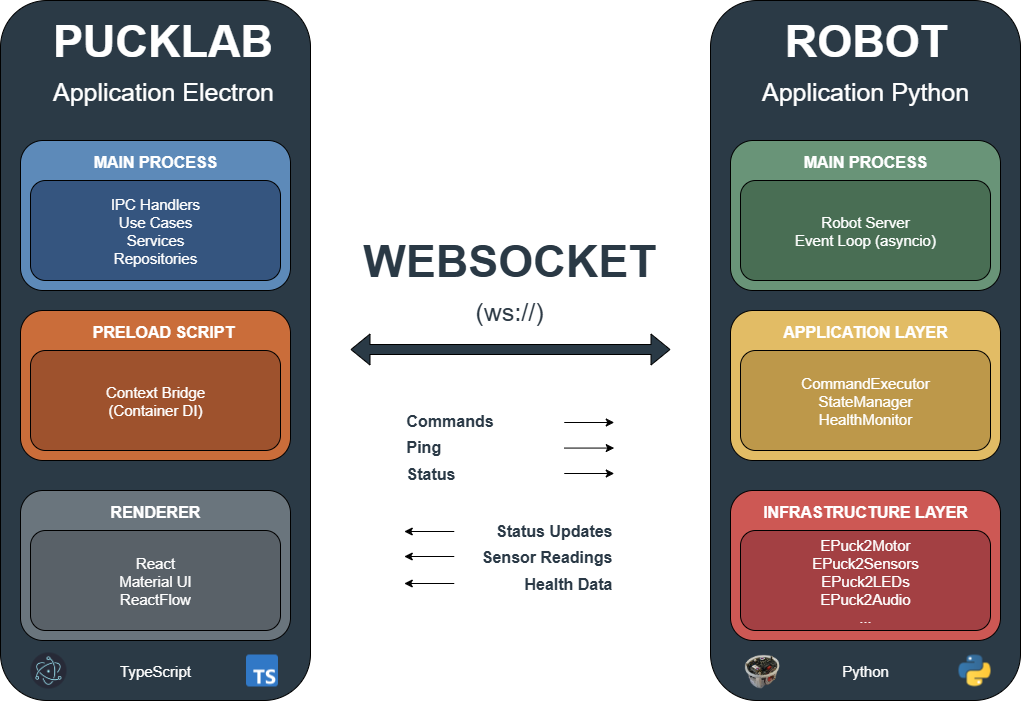
\includegraphics[width=1\linewidth]{figures//implementation-schema.png}
    \caption{\label{fig:structure_interactions} Structure et interactions des codebases}
\end{figure}

\subsection{Développement de l'interface utilisateur (client)}

La première phase a porté sur le développement de l’interface utilisateur avec Electron, en s’appuyant sur React comme moteur de rendu, et sur le langage TypeScript pour bénéficier d’un typage fort assurant une meilleure robustesse du code.

Une attention particulière a été portée à l’implémentation de la \textit{clean architecture}, afin de bien distinguer les responsabilités entre les différentes couches applicatives et leur contexte d’exécution.
En effet, Electron repose sur une séparation stricte entre le \textit{main process} (responsable de la gestion des fenêtres, du système de fichiers, etc.) et le \textit{renderer process} (dédié à l’affichage de l’interface).
Ces deux processus ne pouvant pas interagir directement, un pont de communication a été mis en place via un \textit{context bridge}, étendant l’objet global $Window$ pour exposer une API sécurisée entre les deux contextes.

Une fois cette structure maîtrisée, le développement de l’interface a pu se poursuivre de manière fluide.
Les figures ci-dessous en sont le résultat.

\begin{figure}[H]
    \centering

    \begin{subfigure}{0.45\linewidth}
        \centering
        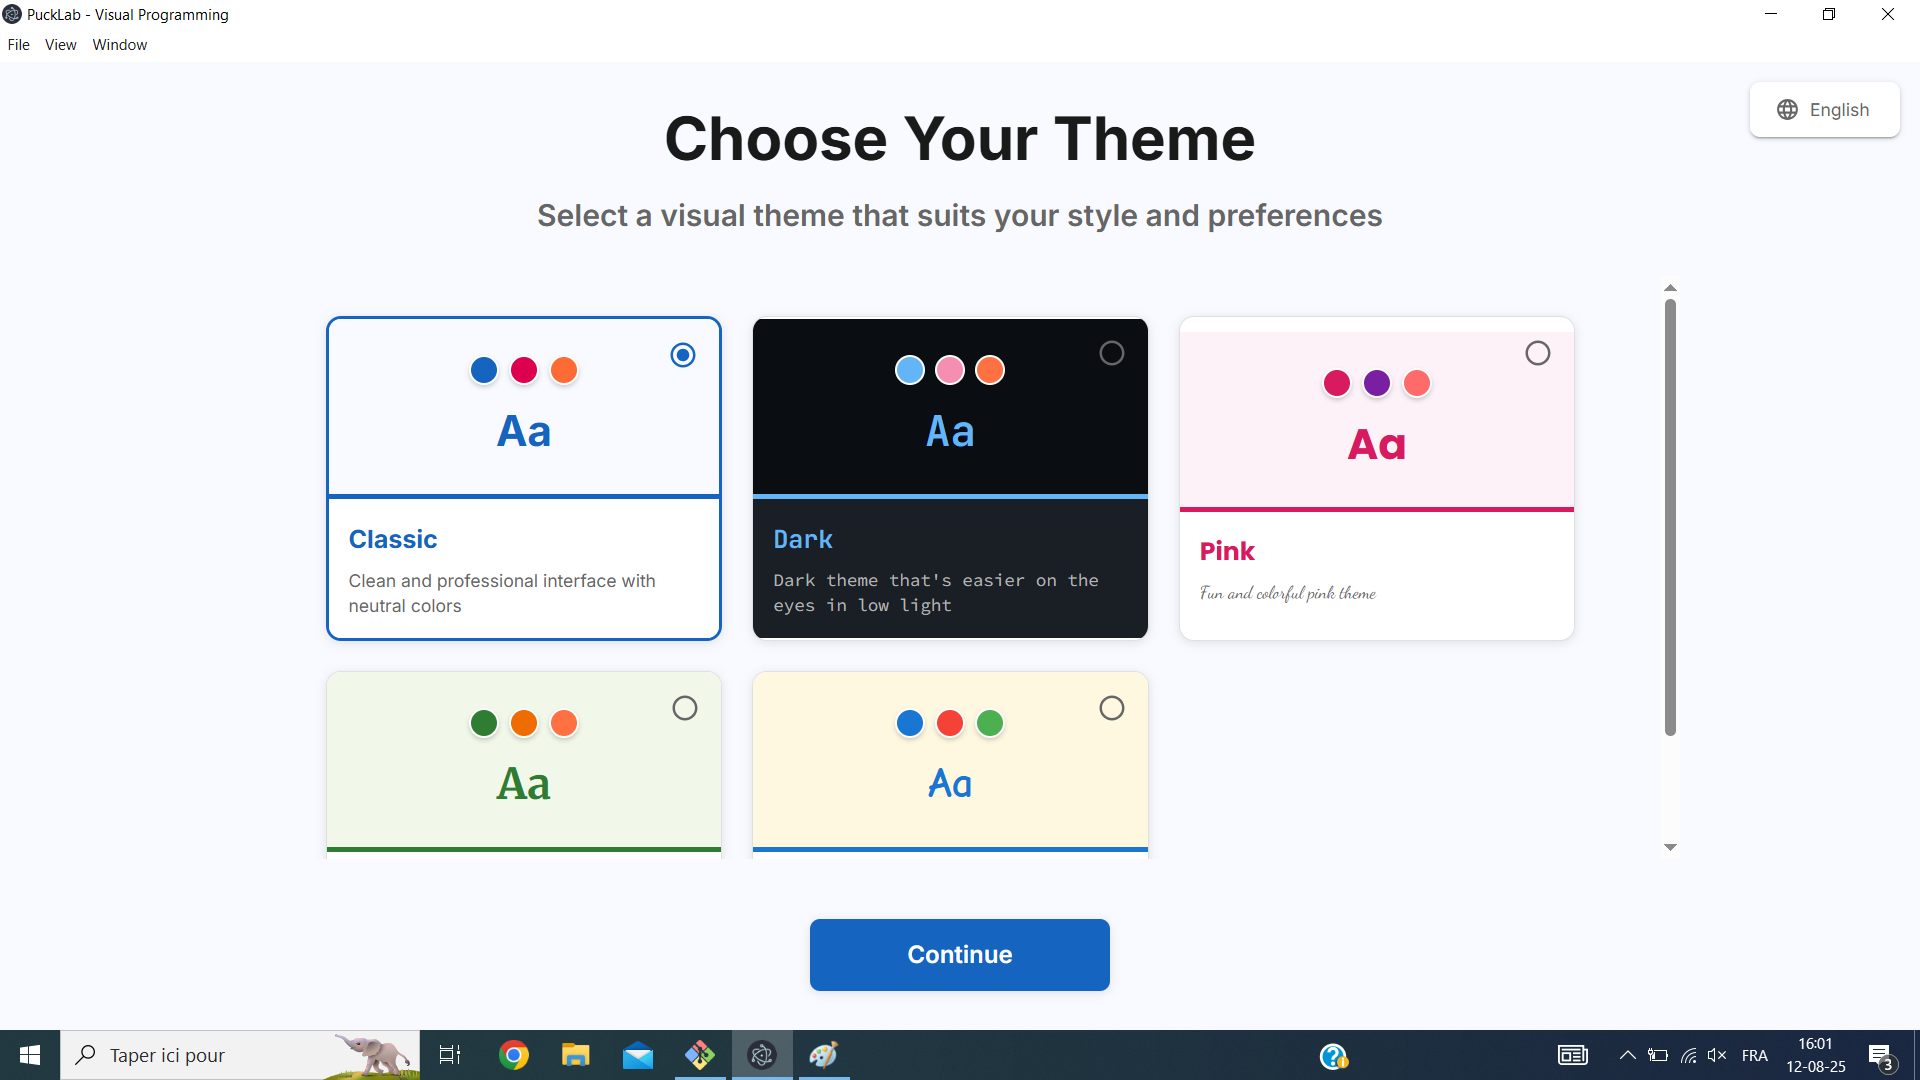
\includegraphics[width=\linewidth]{figures//screenshots//theme choice selection classic.png}
        \caption{\label{fig:classic_theme_choice} Écran - Choix du thème (classique)}
    \end{subfigure}
    \hfill
    \begin{subfigure}{0.45\linewidth}
        \centering
        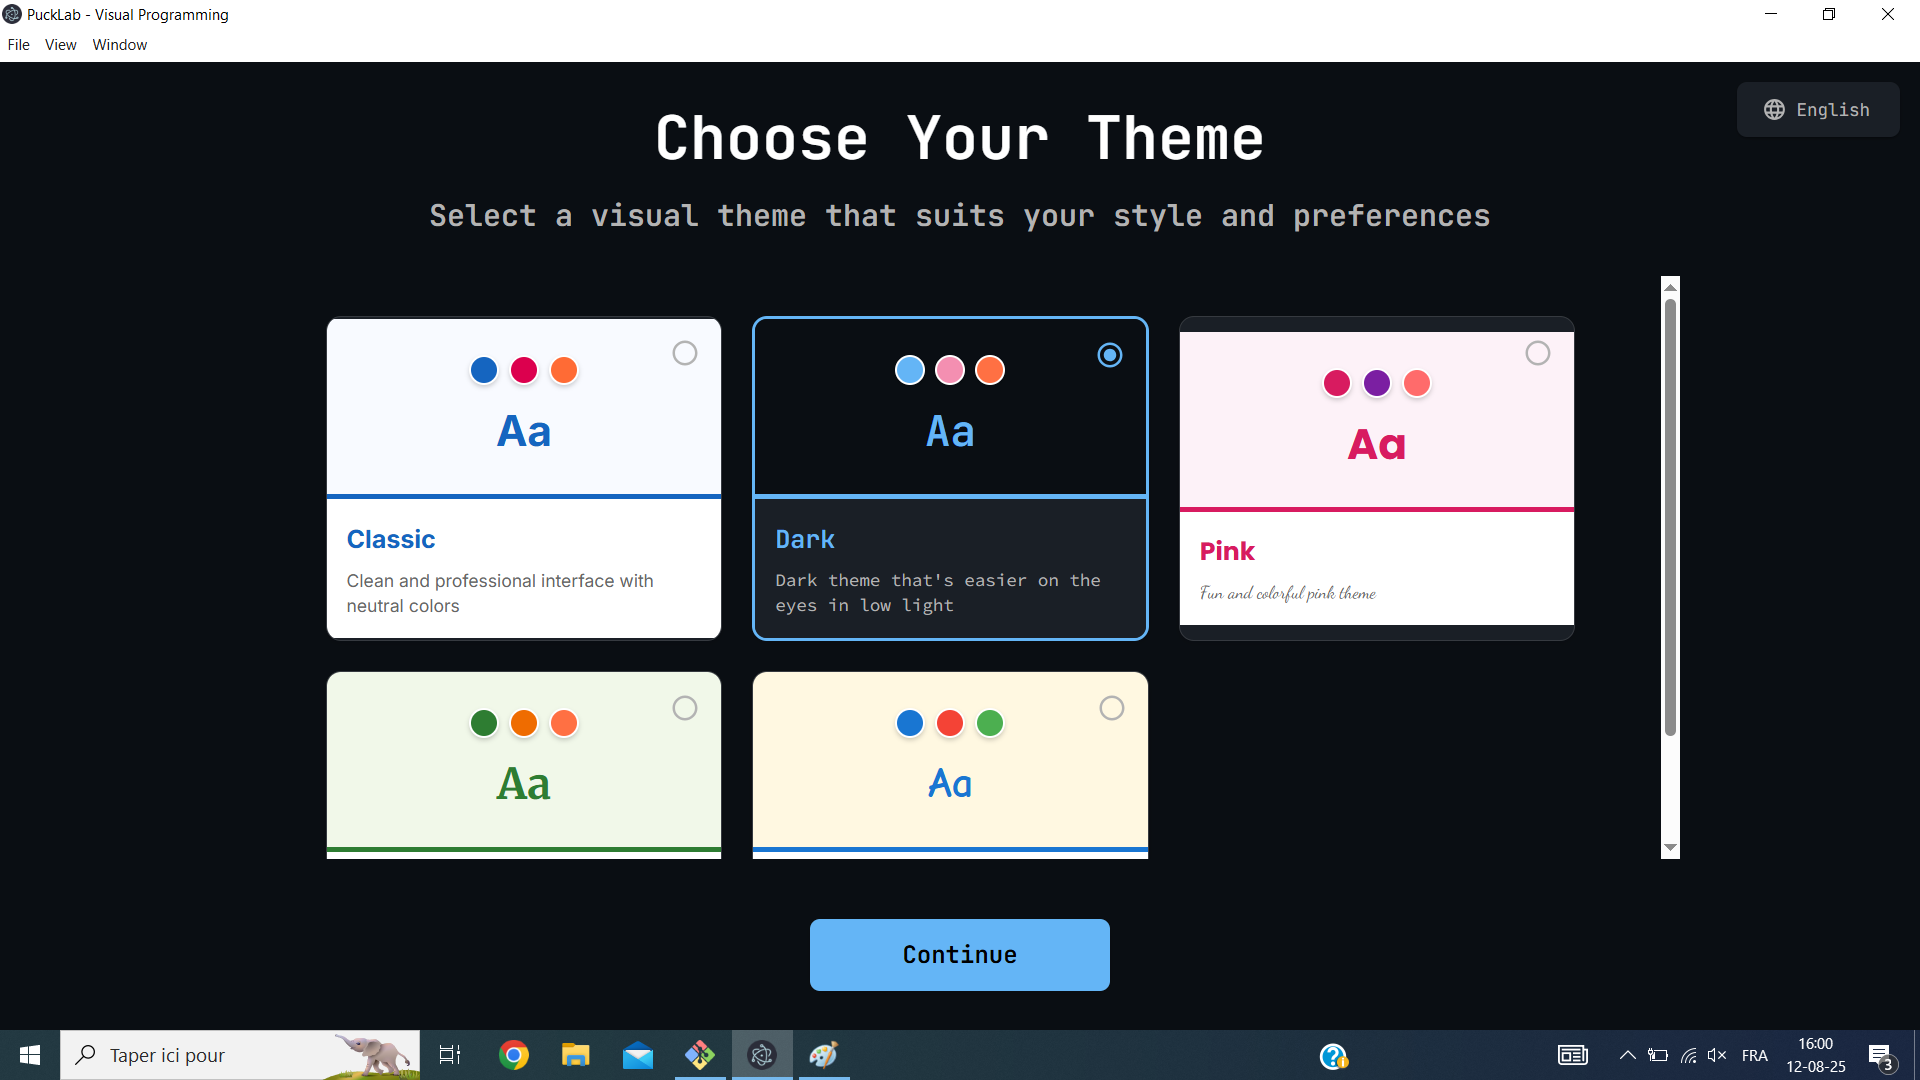
\includegraphics[width=\linewidth]{figures//screenshots//theme choice selection dark.png}
        \caption{\label{fig:dark_theme_choice} Écran - Choix du thème (sombre)}
    \end{subfigure}

    \vspace{0.25cm}

    \begin{subfigure}{0.45\linewidth}
        \centering
        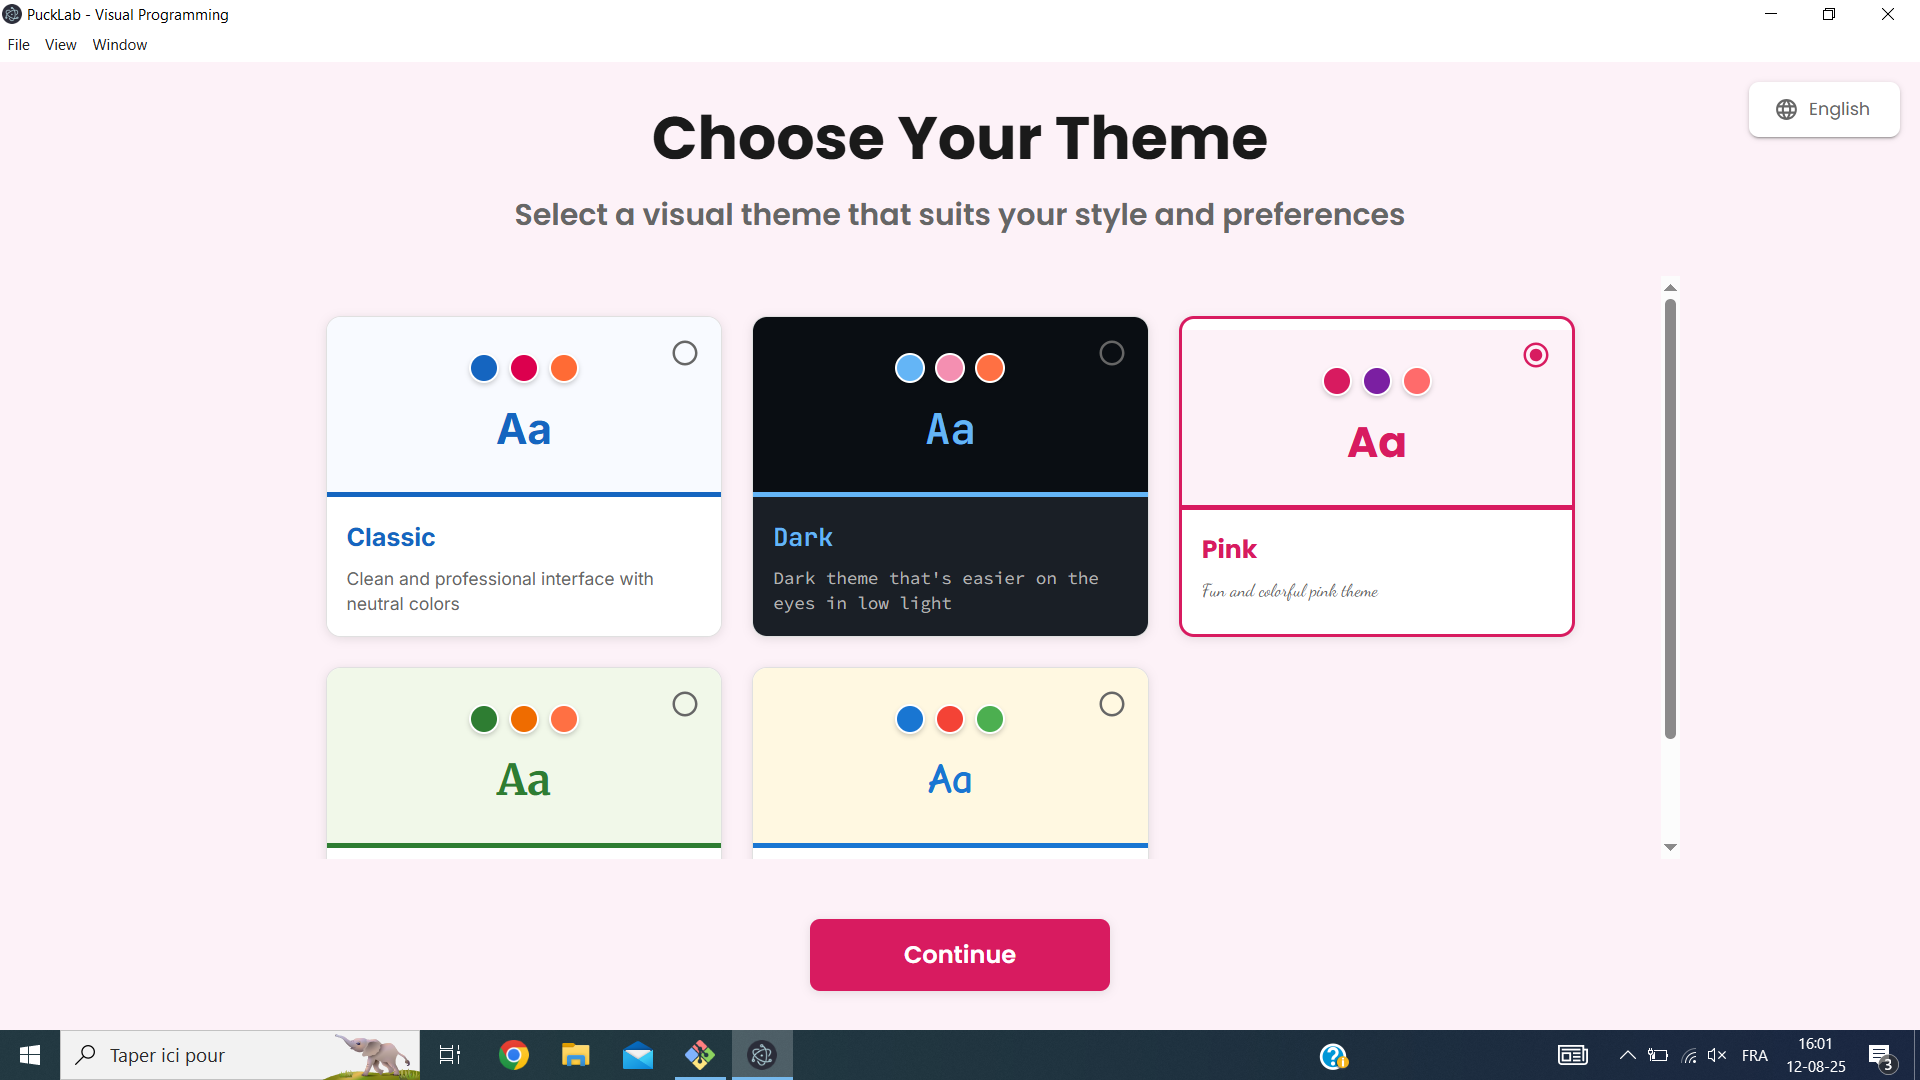
\includegraphics[width=\linewidth]{figures//screenshots//theme choice selection pink.png}
        \caption{\label{fig:pink_theme_choice} Écran - Choix du thème (rose)}
    \end{subfigure}
    \hfill
    \begin{subfigure}{0.45\linewidth}
        \centering
        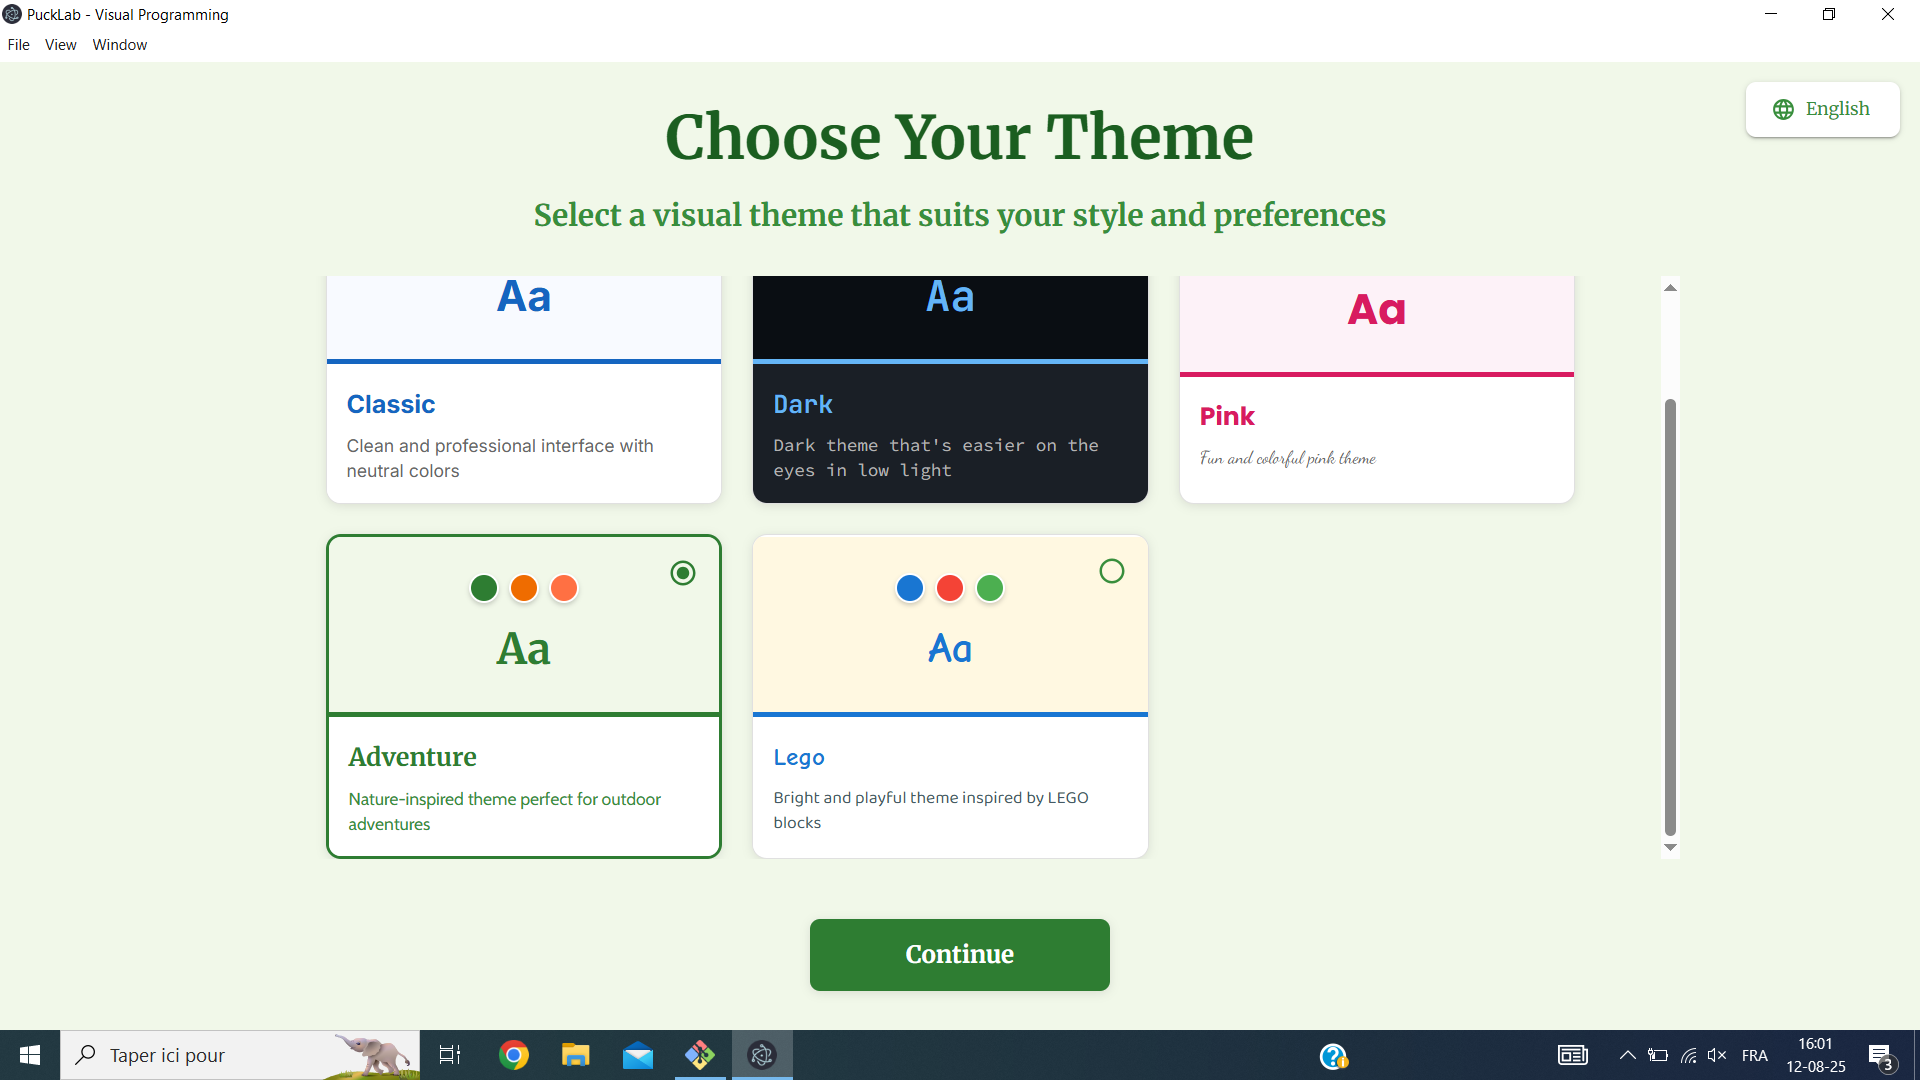
\includegraphics[width=\linewidth]{figures//screenshots//theme choice selection adventure.png}
        \caption{\label{fig:adventure_theme_choice} Écran - Choix du thème (aventure}
    \end{subfigure}

    \vspace{0.25cm}

    \begin{subfigure}{0.45\linewidth}
        \centering
        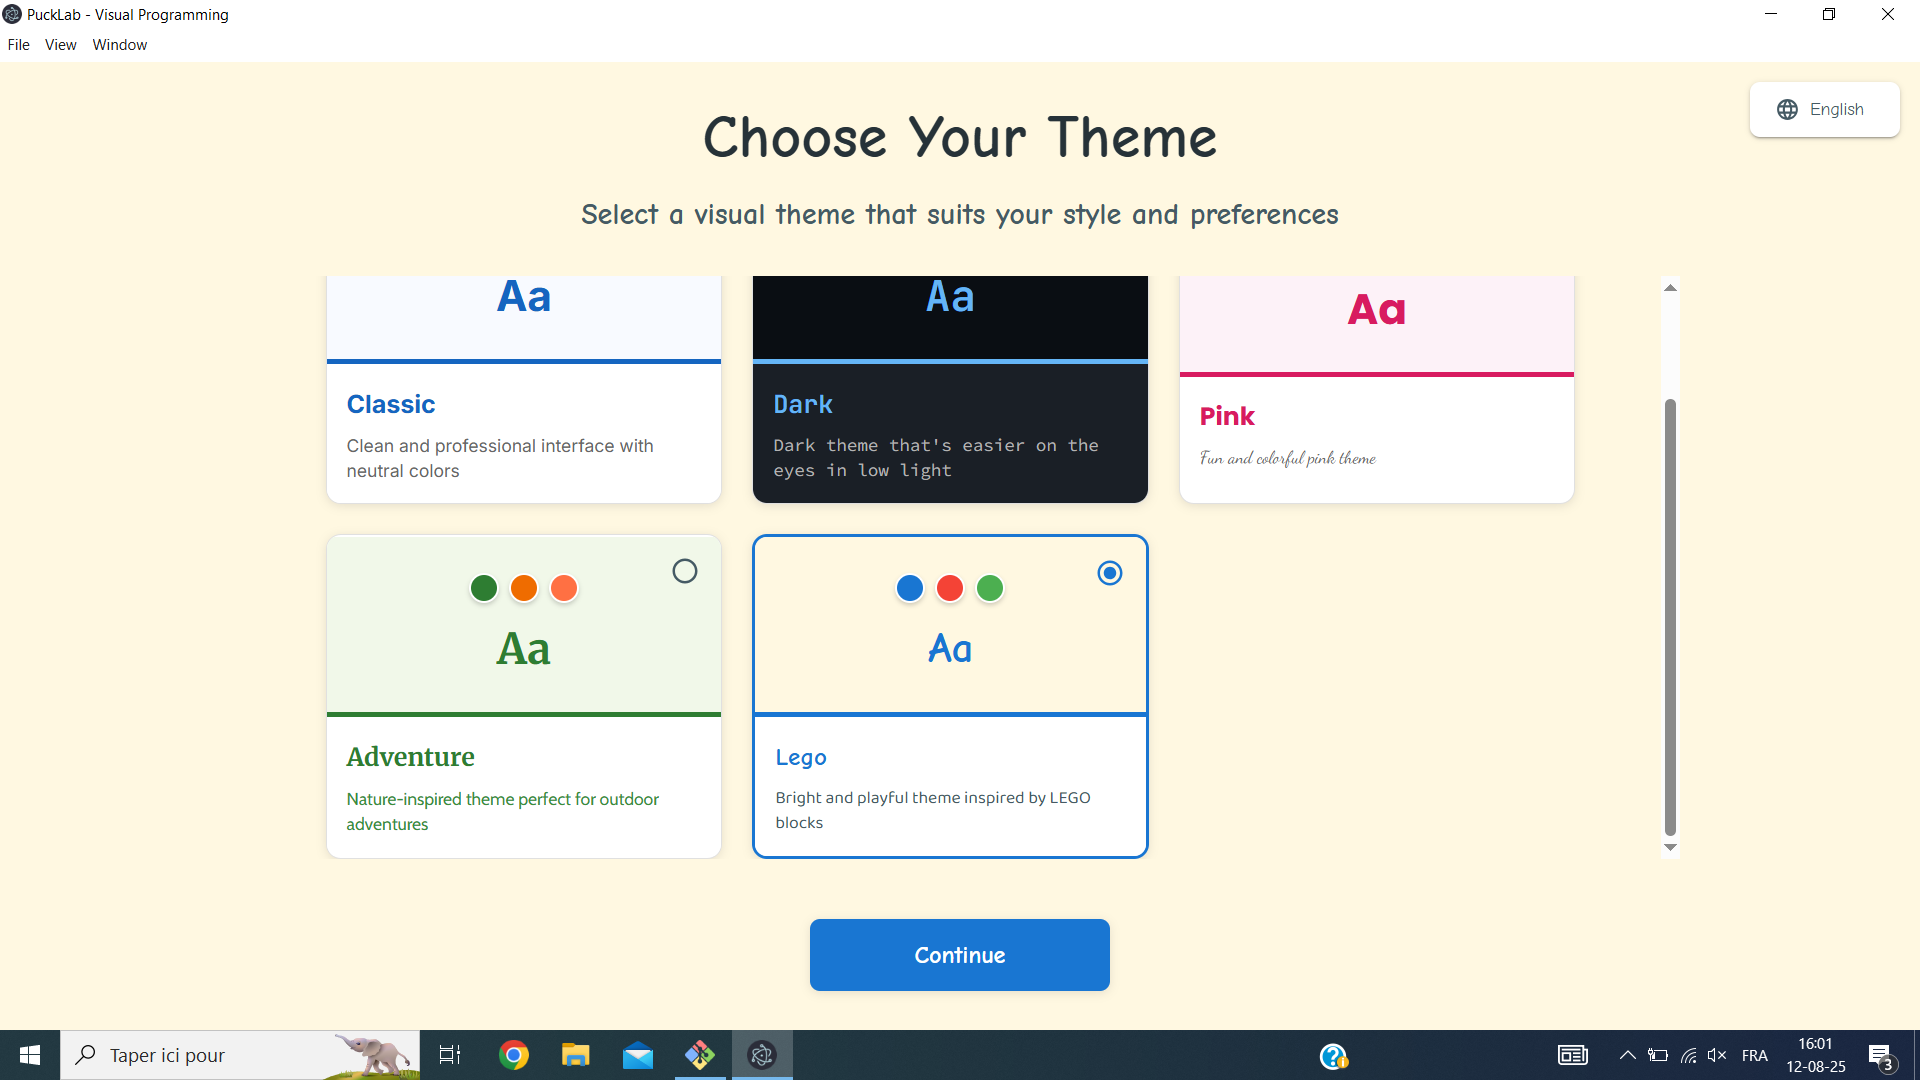
\includegraphics[width=\linewidth]{figures//screenshots//theme choice selection lego.png}
        \caption{\label{fig:lego_theme_choice} Écran - Choix du thème (Lego)}
    \end{subfigure}
    \hfill
    \begin{subfigure}{0.45\linewidth}
        \centering
        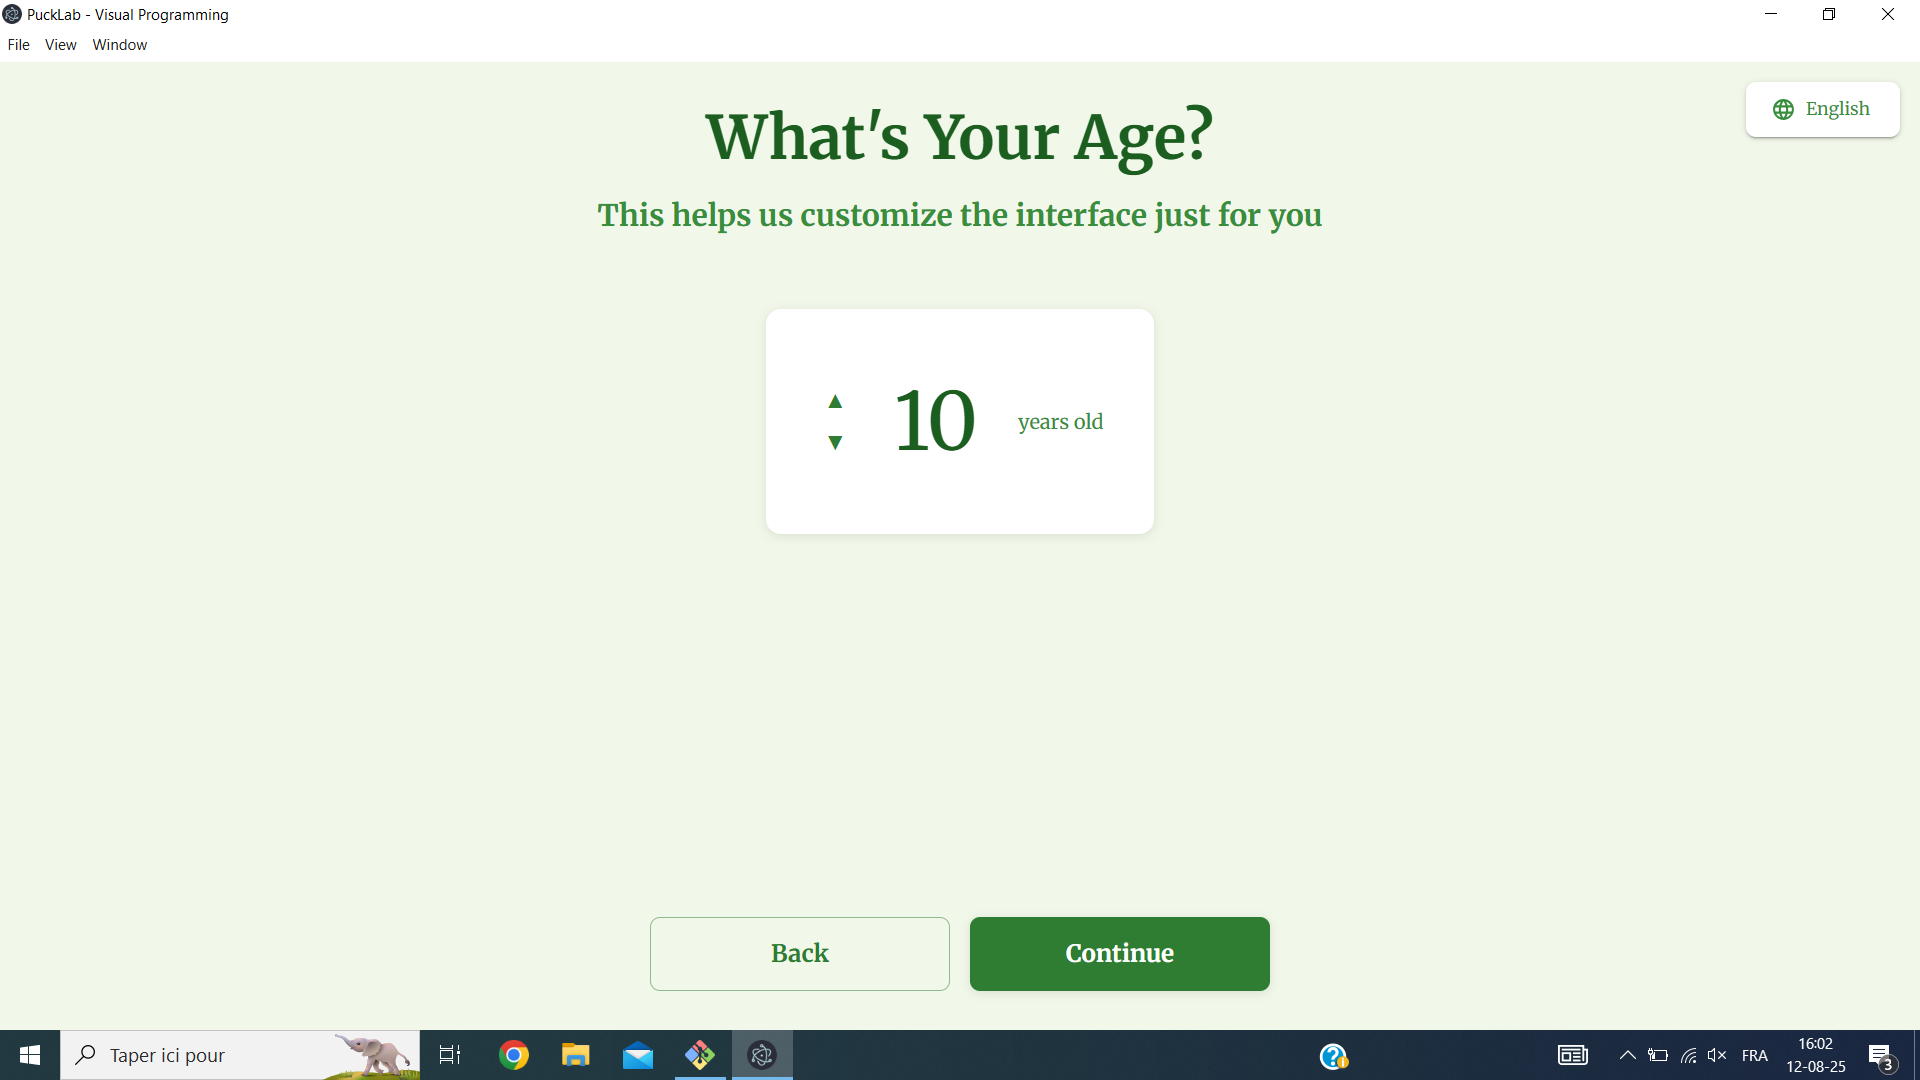
\includegraphics[width=\linewidth]{figures//screenshots//age choice selection.png}
        \caption{\label{fig:age_choice} Écran - Choix de l'âge}
    \end{subfigure}

    \caption{\label{fig:screenshots-1} Captures d'écran de l'application Pucklab - 1}
\end{figure}

\begin{figure}[H]
    \centering

    \begin{subfigure}{0.45\linewidth}
        \centering
        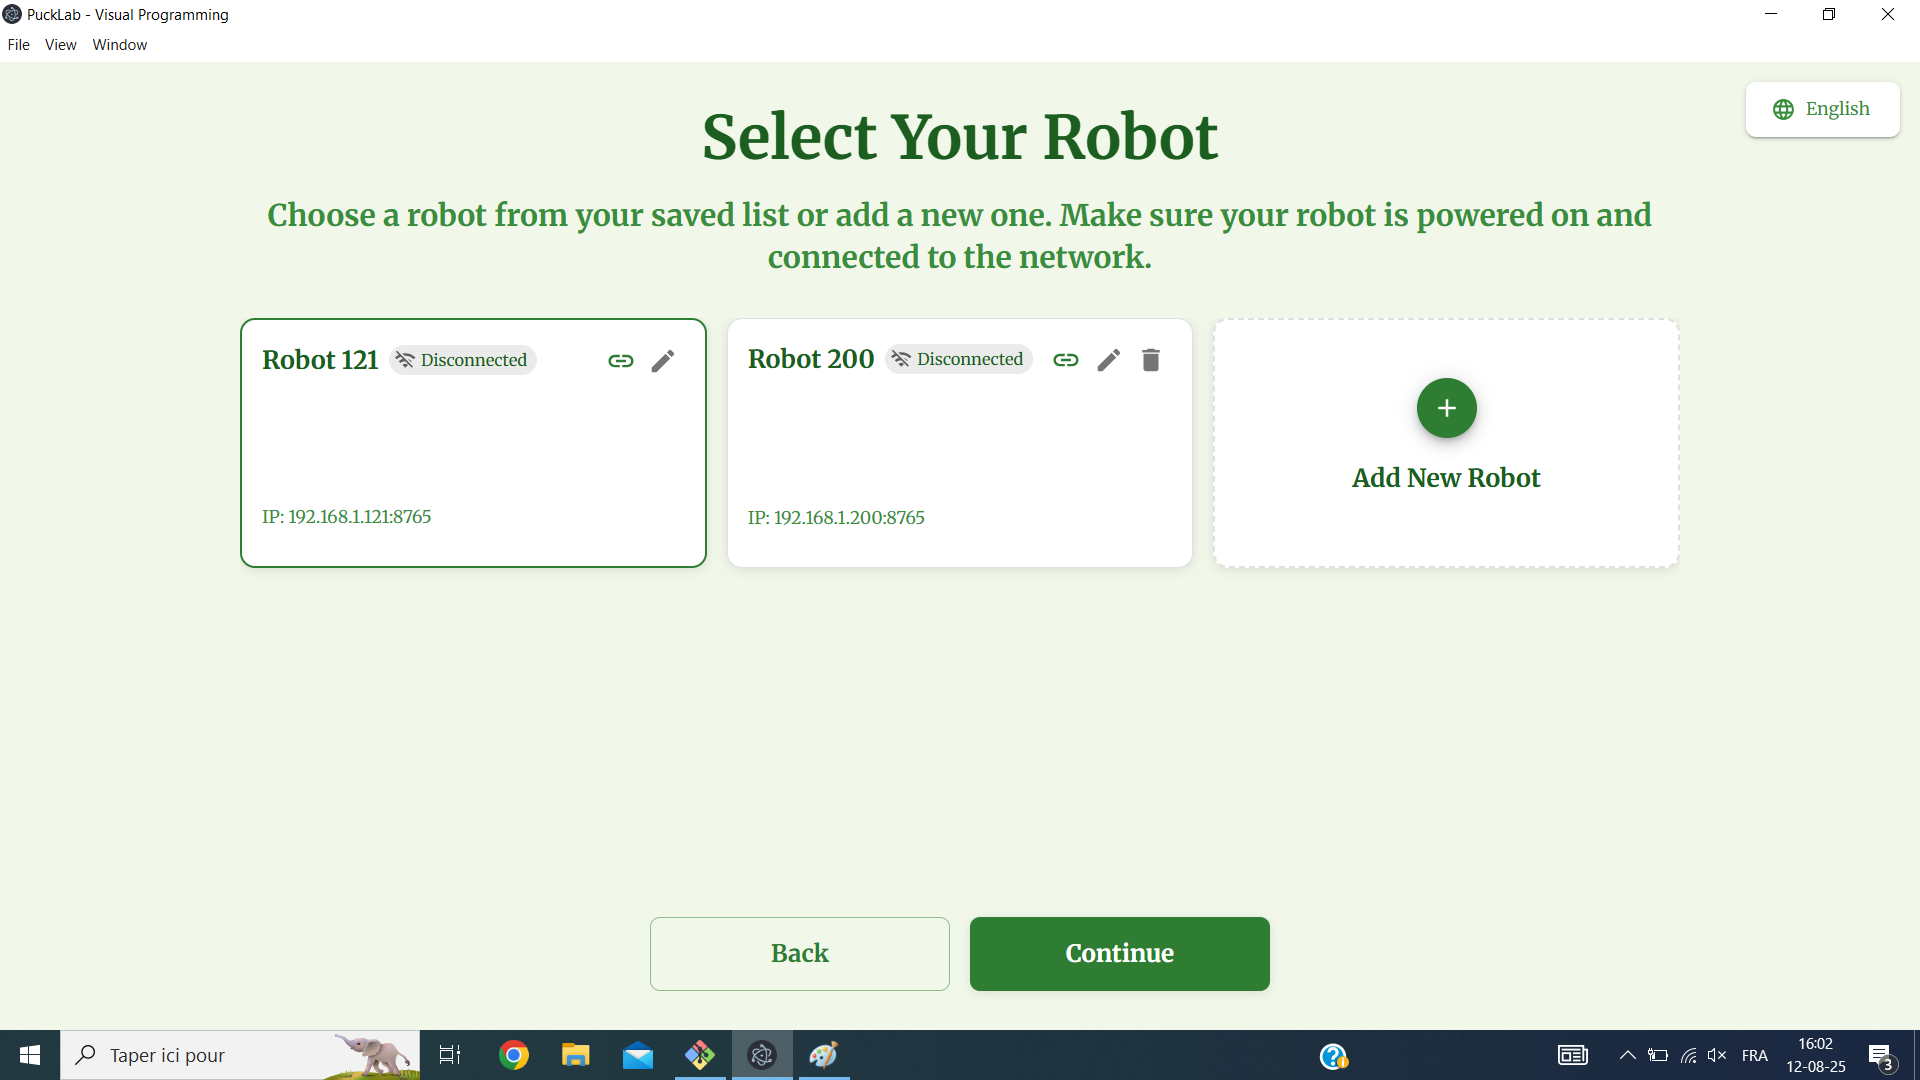
\includegraphics[width=\linewidth]{figures//screenshots//robot choice selection.png}
        \caption{\label{fig:robot_choice} Écran - Choix du robot}
    \end{subfigure}
    \hfill
    \begin{subfigure}{0.45\linewidth}
        \centering
        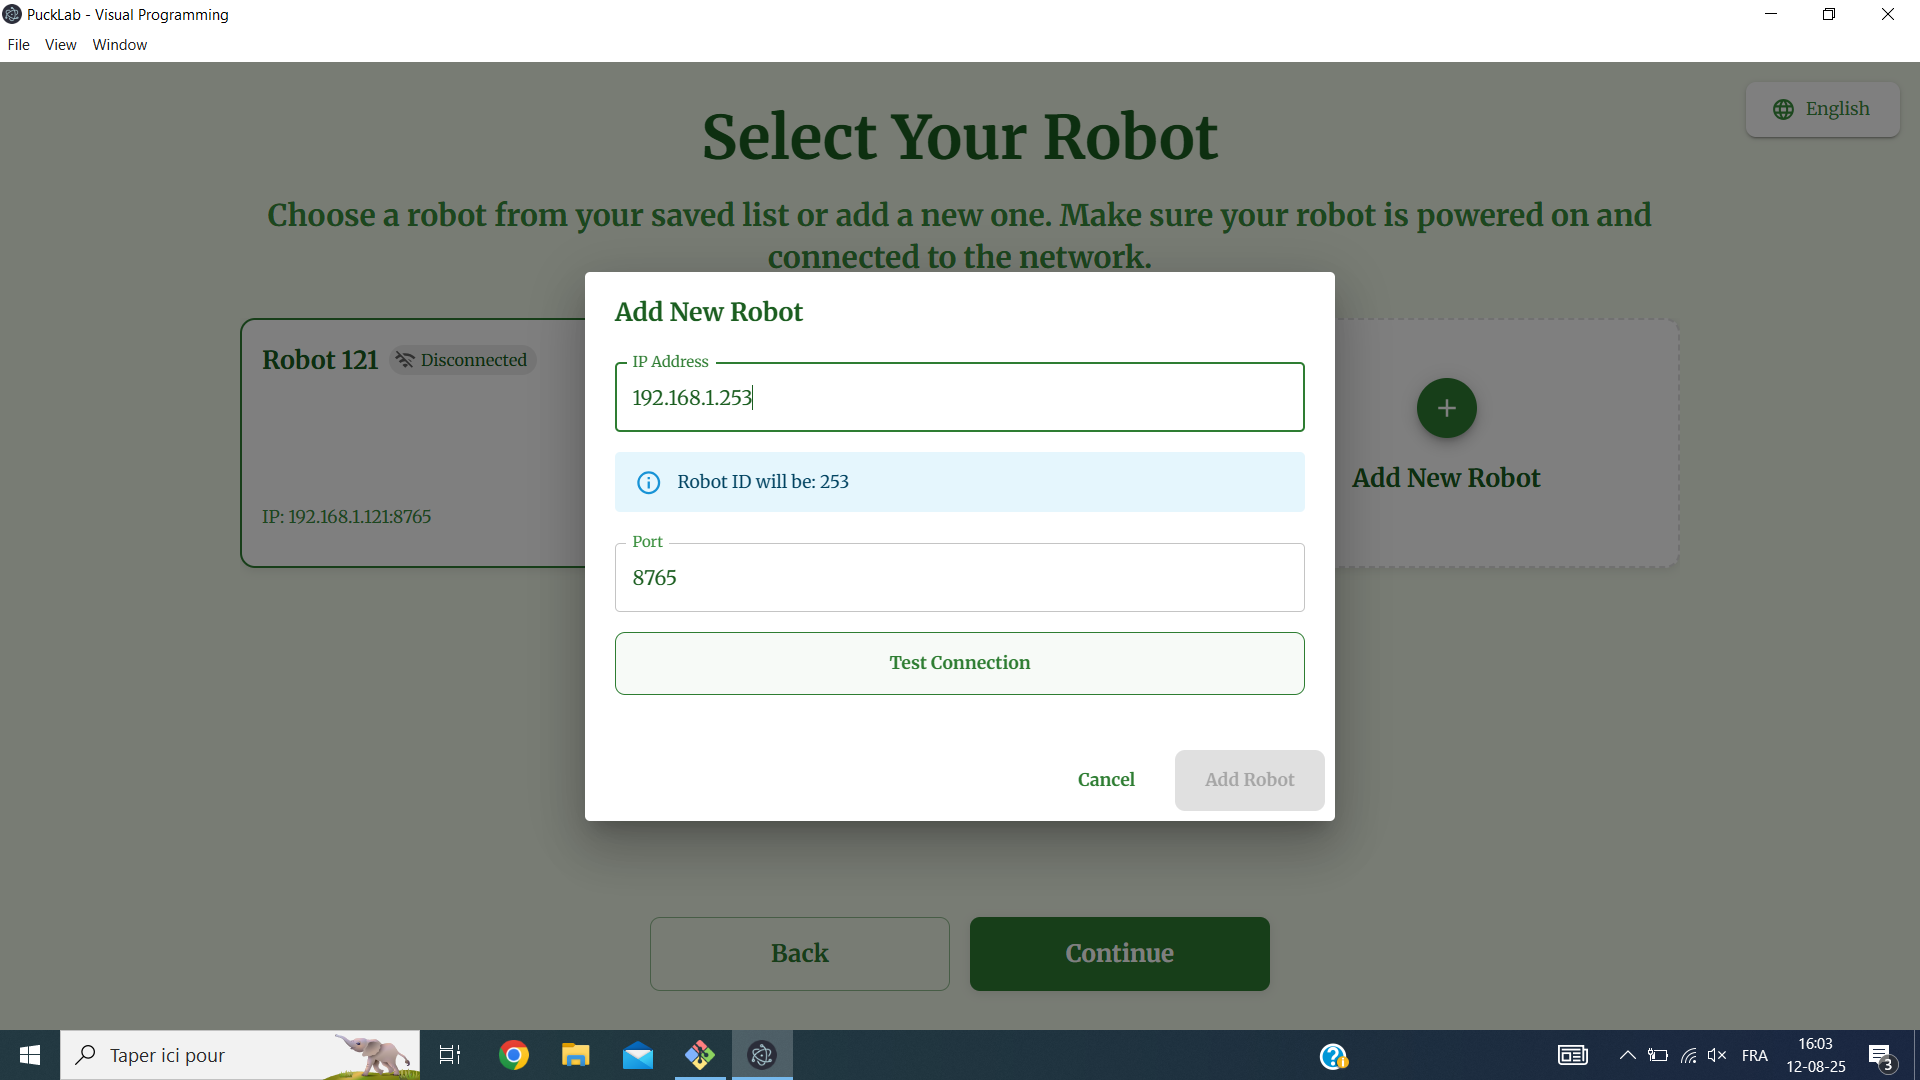
\includegraphics[width=\linewidth]{figures//screenshots//add new robot.png}
        \caption{\label{fig:add_robot_dialog} Écran - Création d'un robot}
    \end{subfigure}

    \vspace{0.25cm}

    \begin{subfigure}{0.45\linewidth}
        \centering
        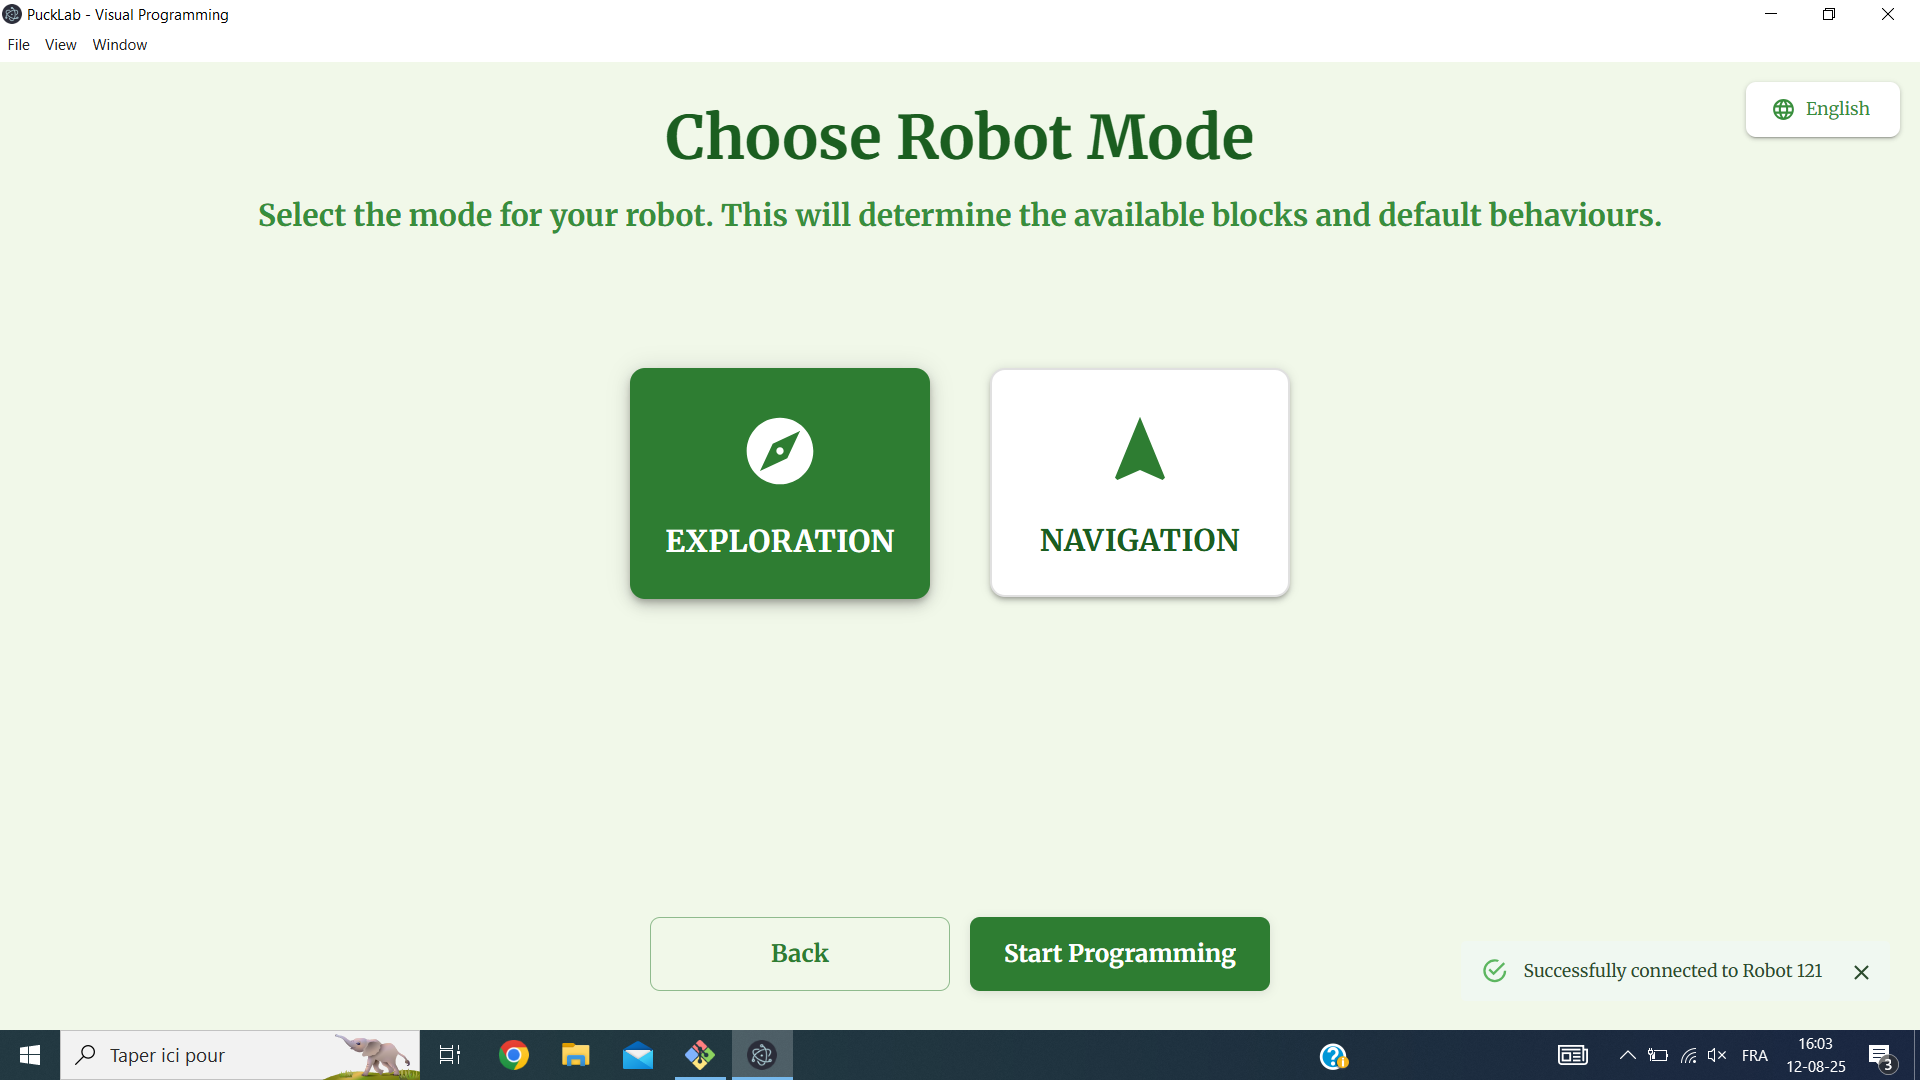
\includegraphics[width=\linewidth]{figures//screenshots//mode choice selection.png}
        \caption{\label{fig:mode_choice} Écran - Choix du mode}
    \end{subfigure}
    \hfill
    \begin{subfigure}{0.45\linewidth}
        \centering
        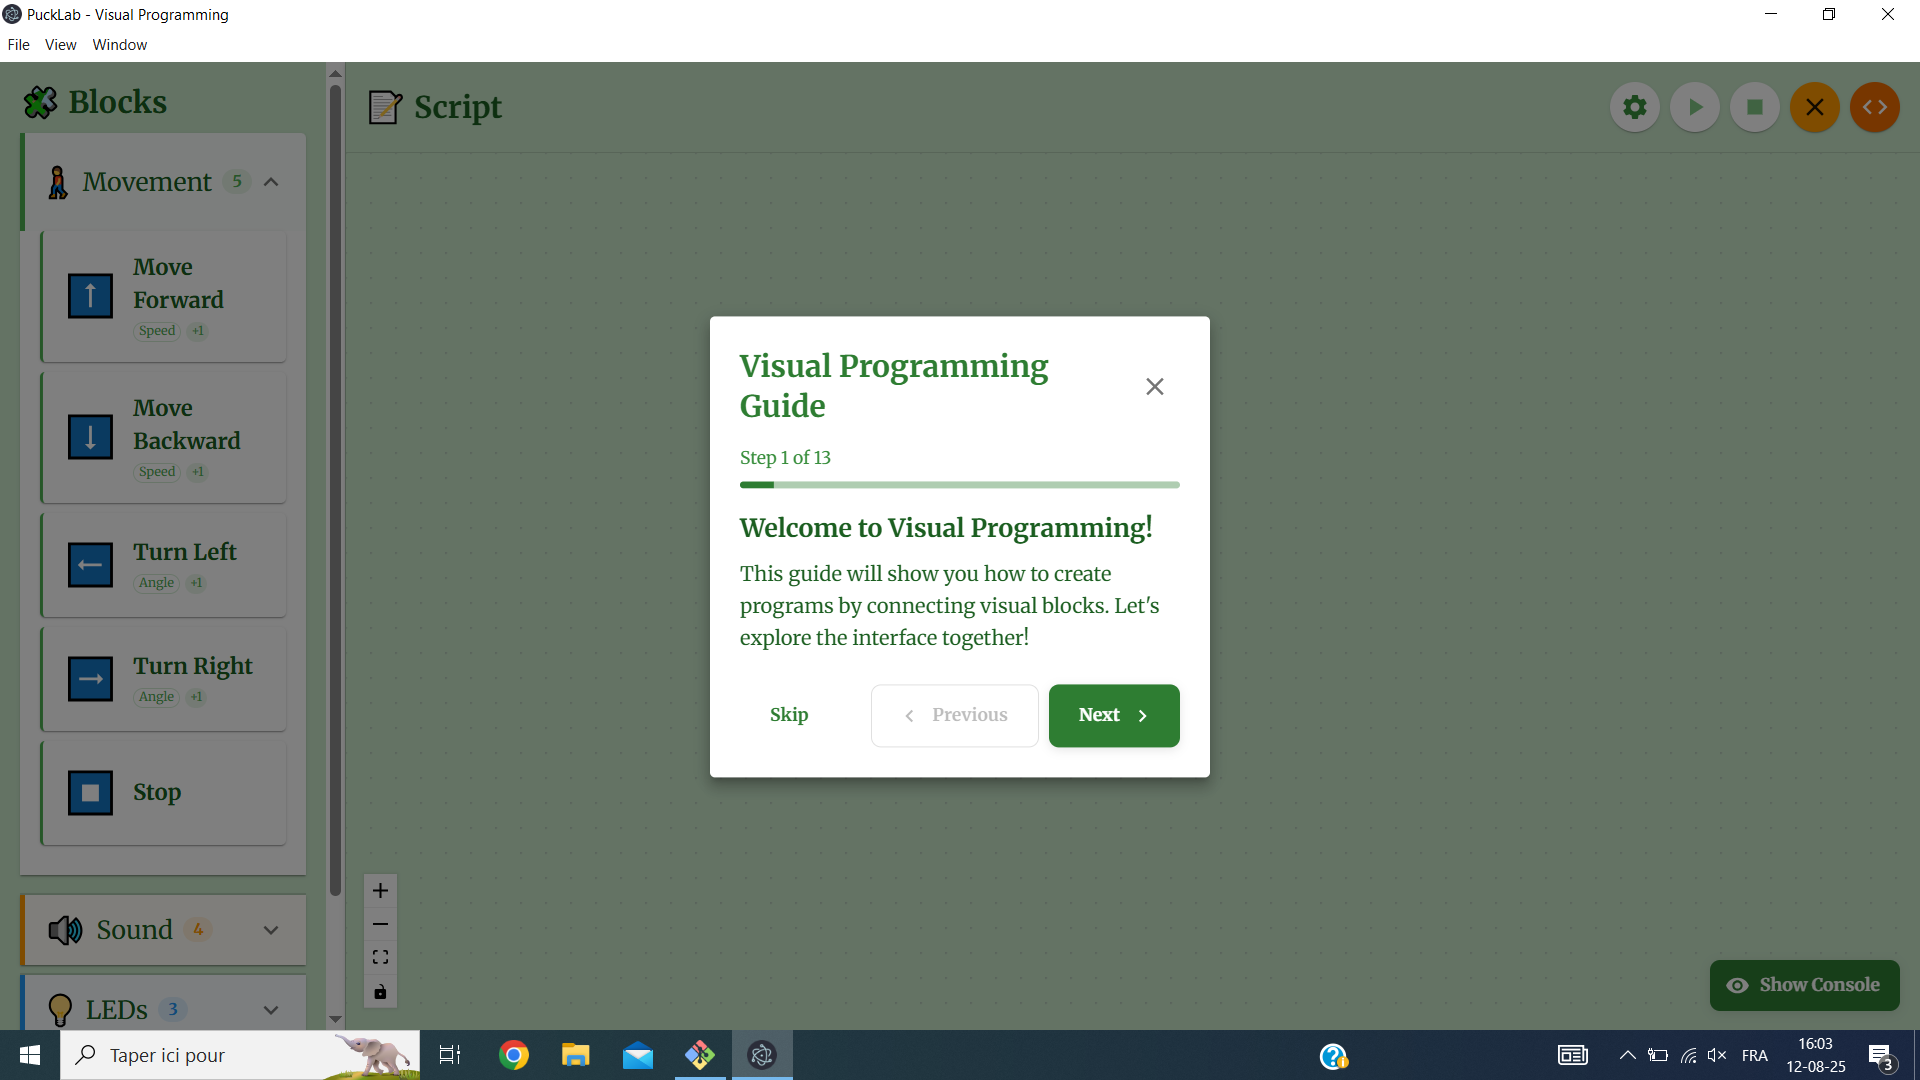
\includegraphics[width=\linewidth]{figures//screenshots//visual programming - age under 12 - tutorial overlay activated.png}
        \caption{\label{fig:vp_ageunder12_tutoactivated} Écran - Programmation Visuelle (jeune - tutorial actif)}
    \end{subfigure}

    \vspace{0.25cm}

    \begin{subfigure}{0.45\linewidth}
        \centering
        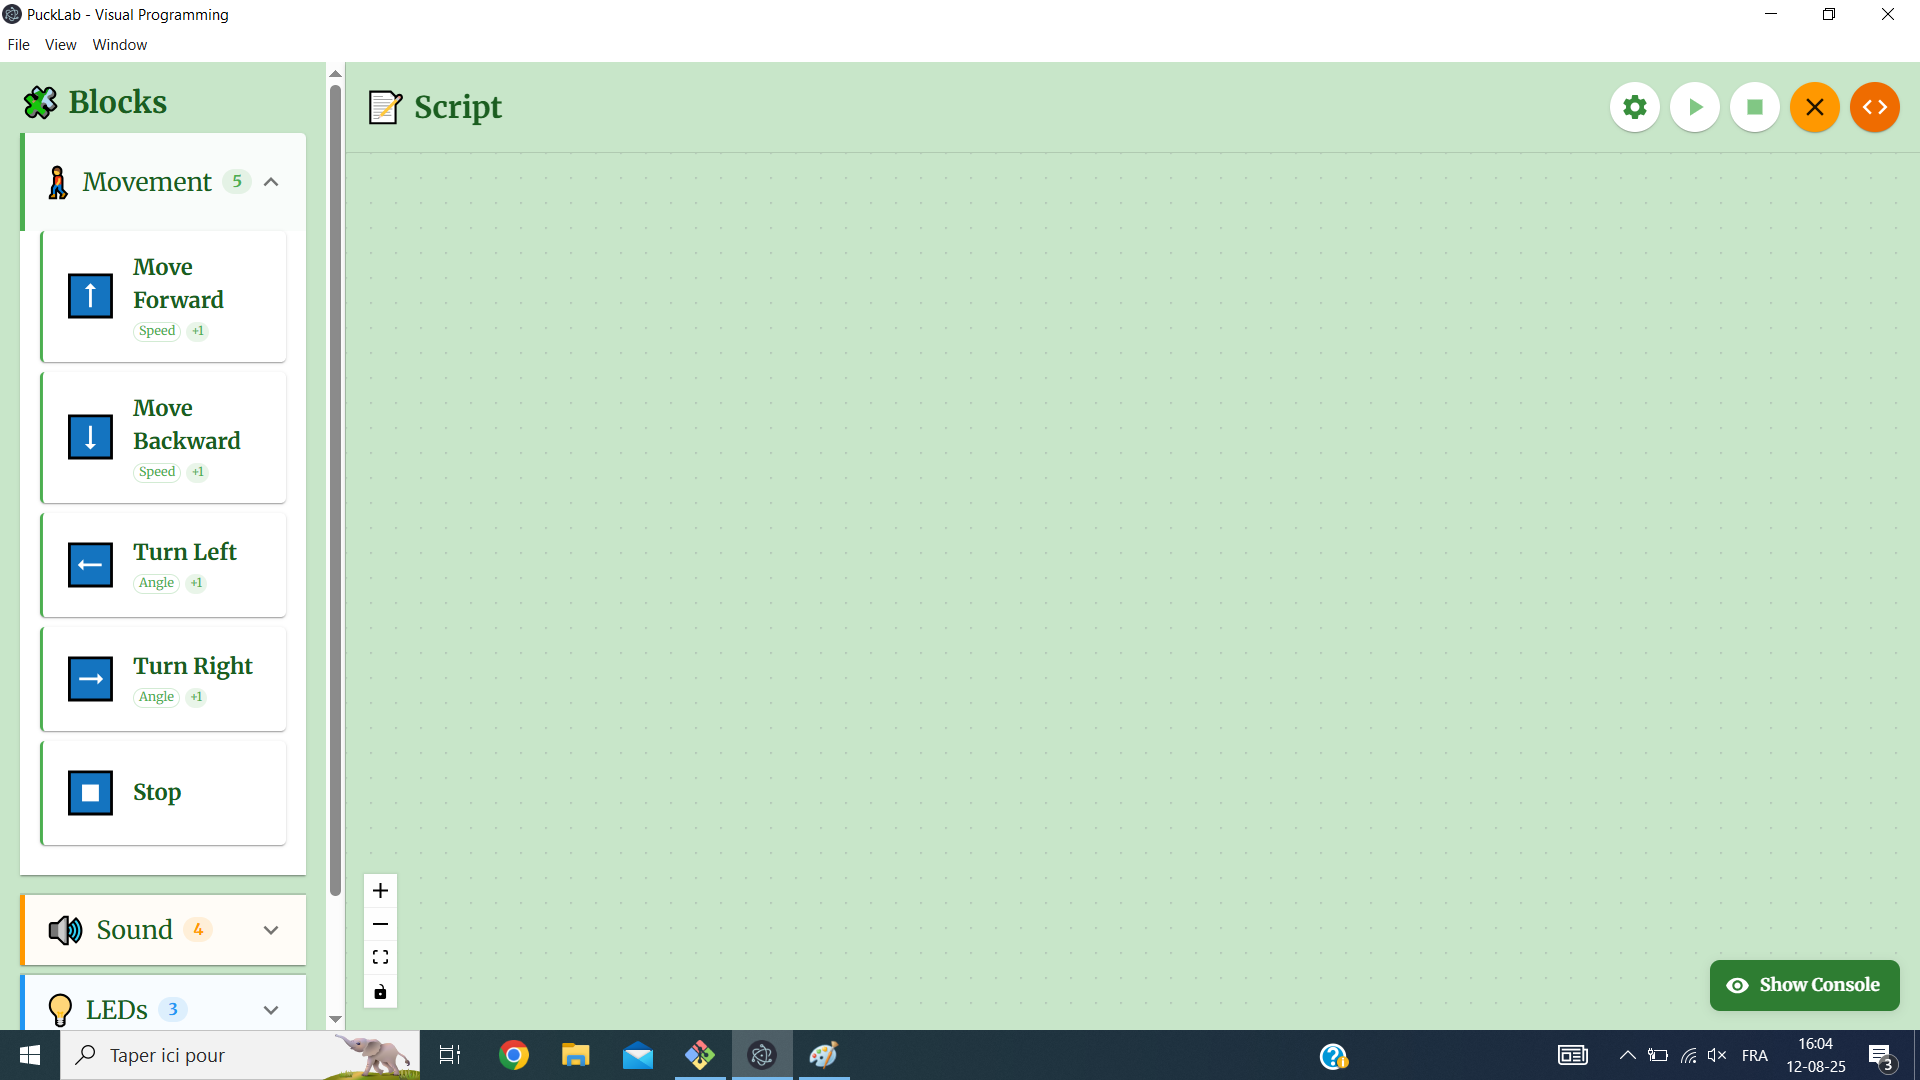
\includegraphics[width=\linewidth]{figures//screenshots//visual programming - age under 12.png}
        \caption{\label{fig:vp_ageunder12} Écran - Programmation Visuelle (jeune)}
    \end{subfigure}
    \hfill
    \begin{subfigure}{0.45\linewidth}
        \centering
        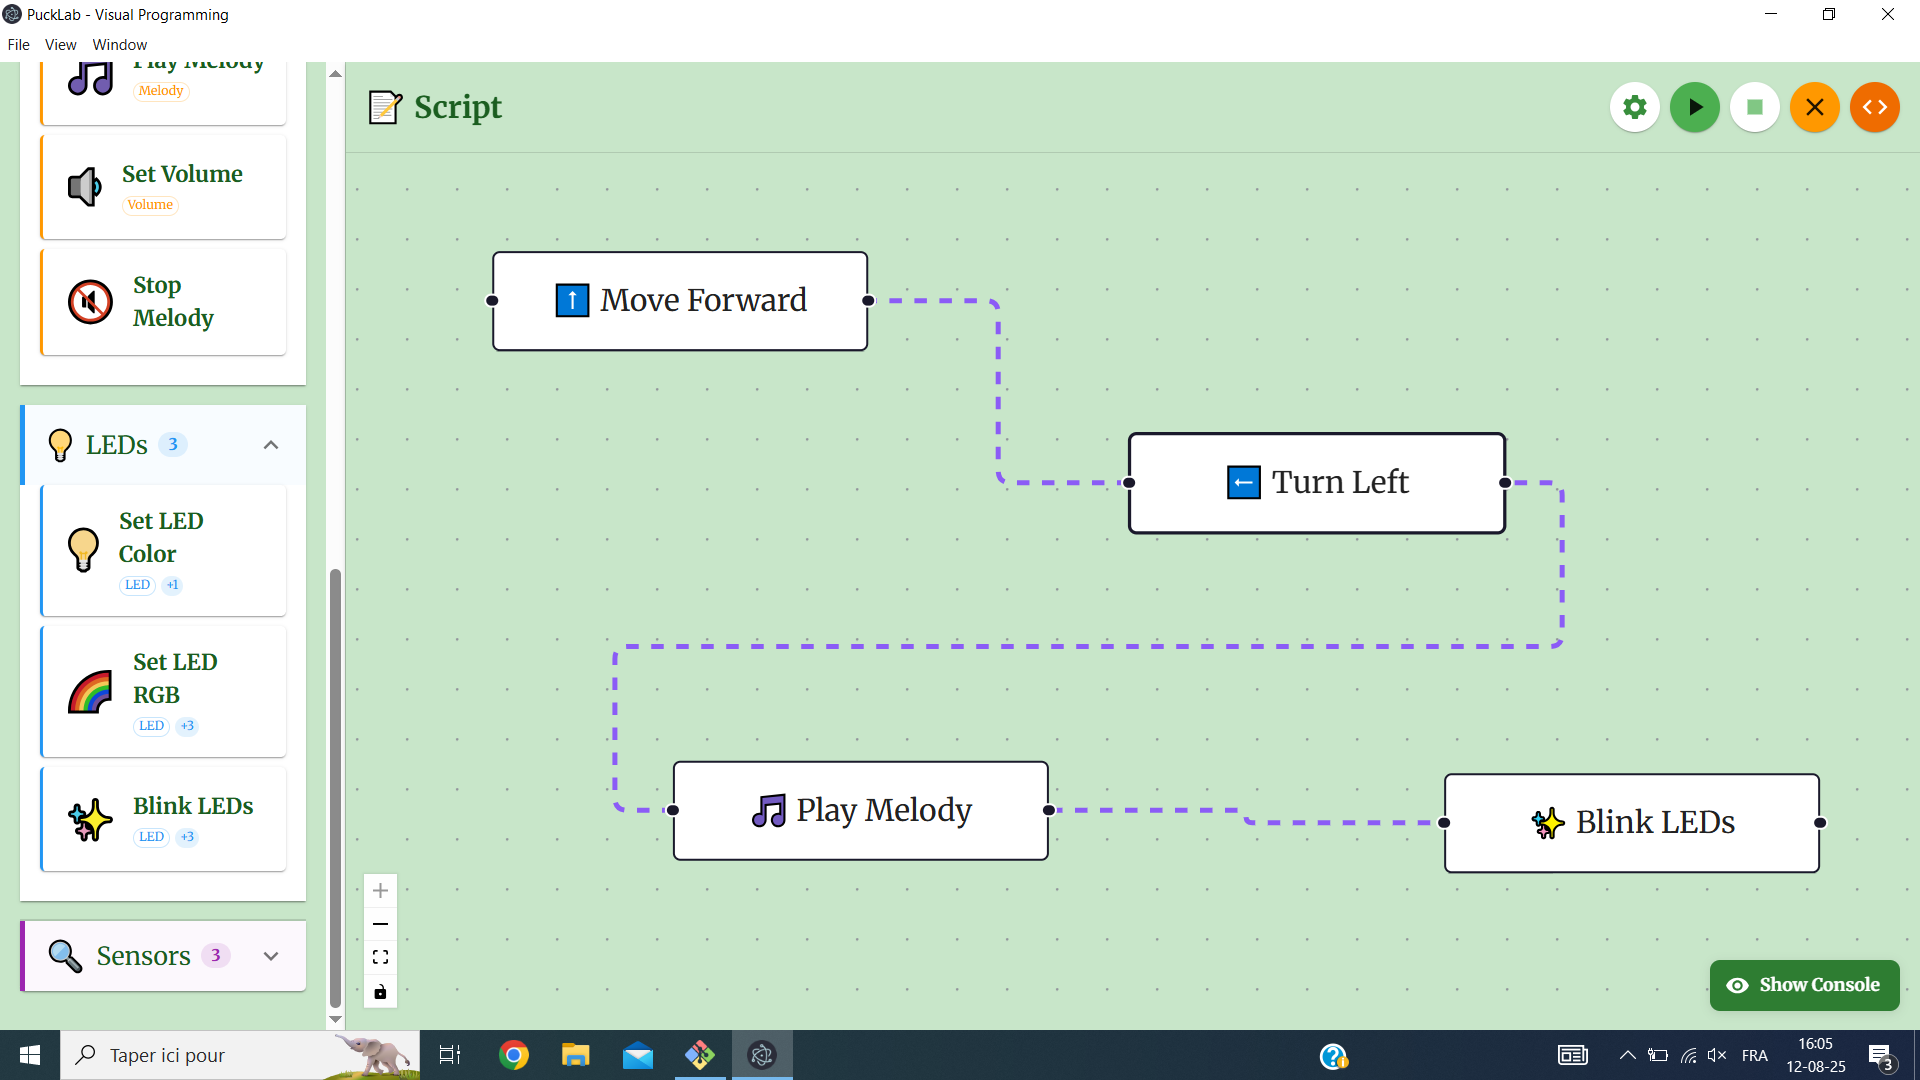
\includegraphics[width=\linewidth]{figures//screenshots//visual programming - age under 12 - basic script.png}
        \caption{\label{fig:vp_ageunder12_basic script} Écran - Programmation Visuelle (jeune - script basique)}
    \end{subfigure}

    \vspace{0.25cm}

    \begin{subfigure}{0.45\linewidth}
        \centering
        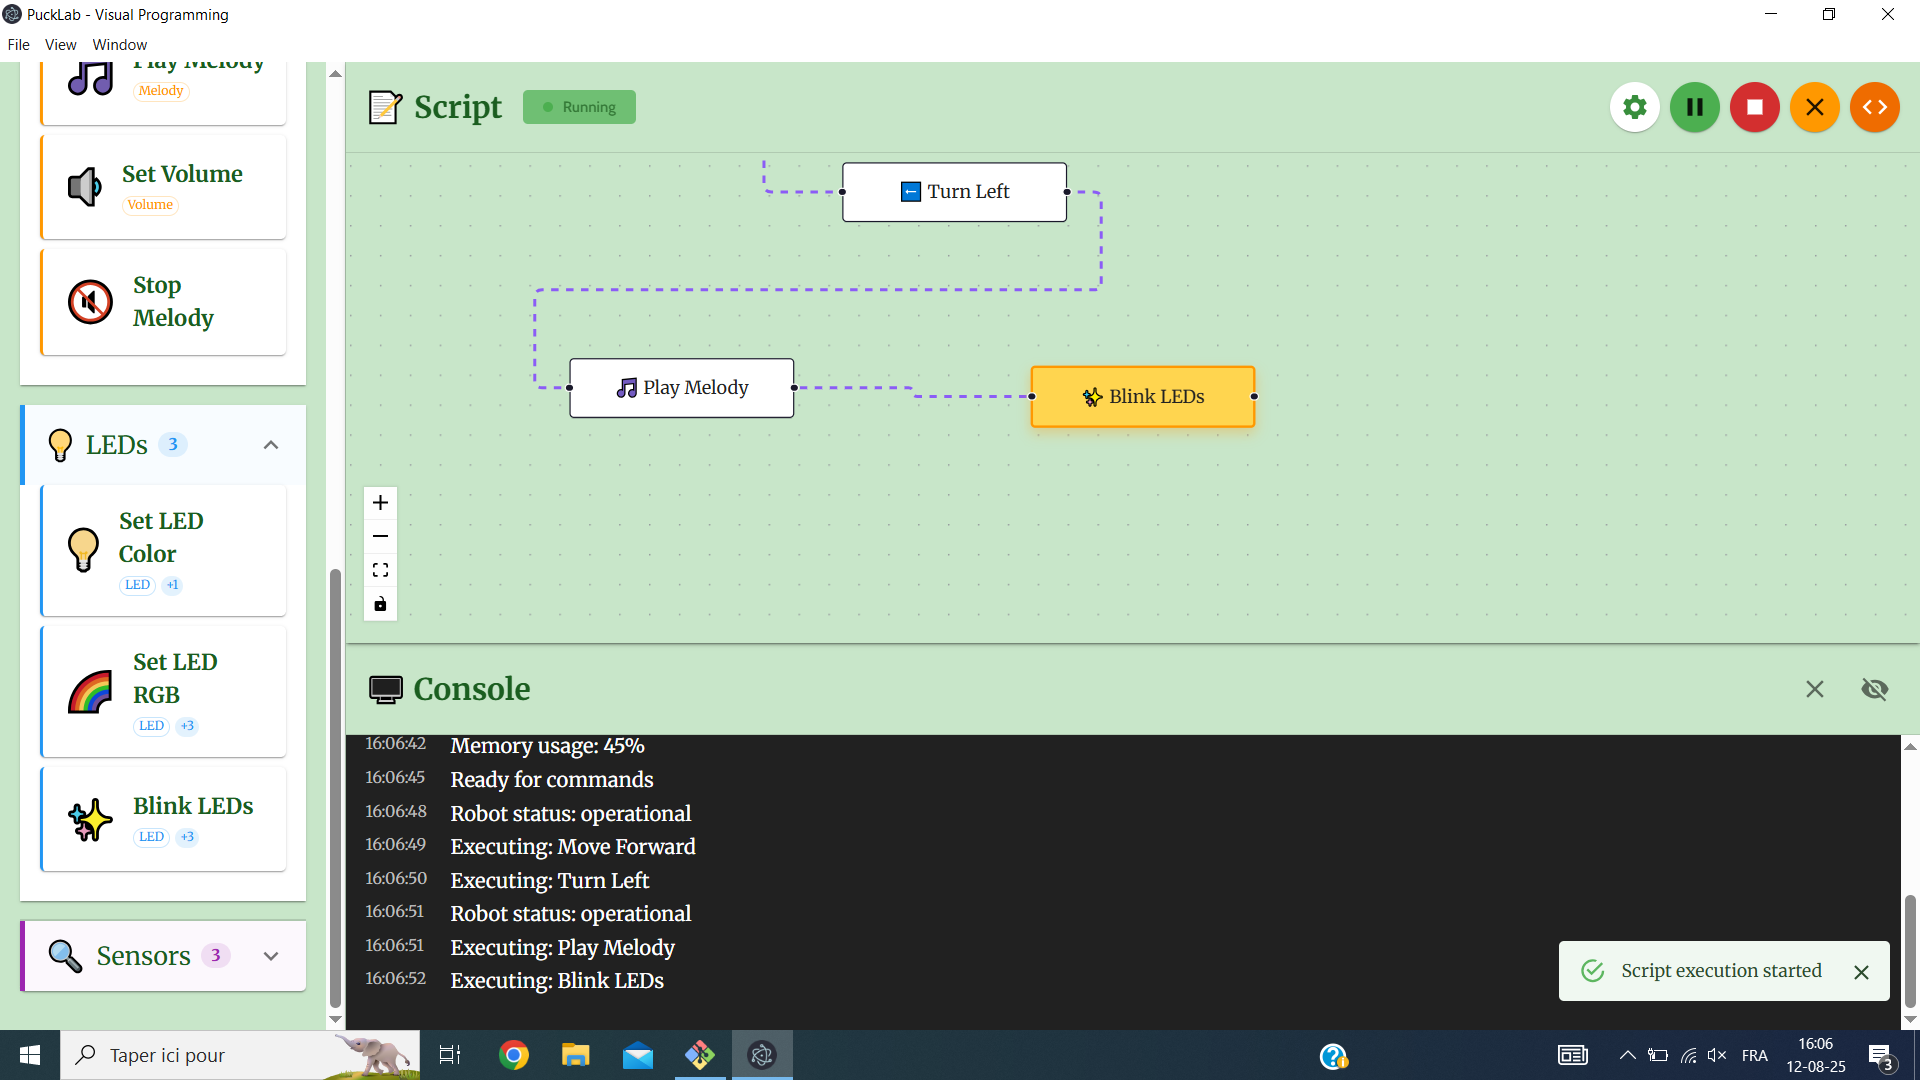
\includegraphics[width=\linewidth]{figures//screenshots//visual programming - age under 12 - basic script executing.png}
        \caption{\label{fig:vp_ageunder12_basicscriptexecuting} Écran - Programmation Visuelle (jeune - script basique en exécution)}
    \end{subfigure}
    \hfill
    \begin{subfigure}{0.45\linewidth}
        \centering
        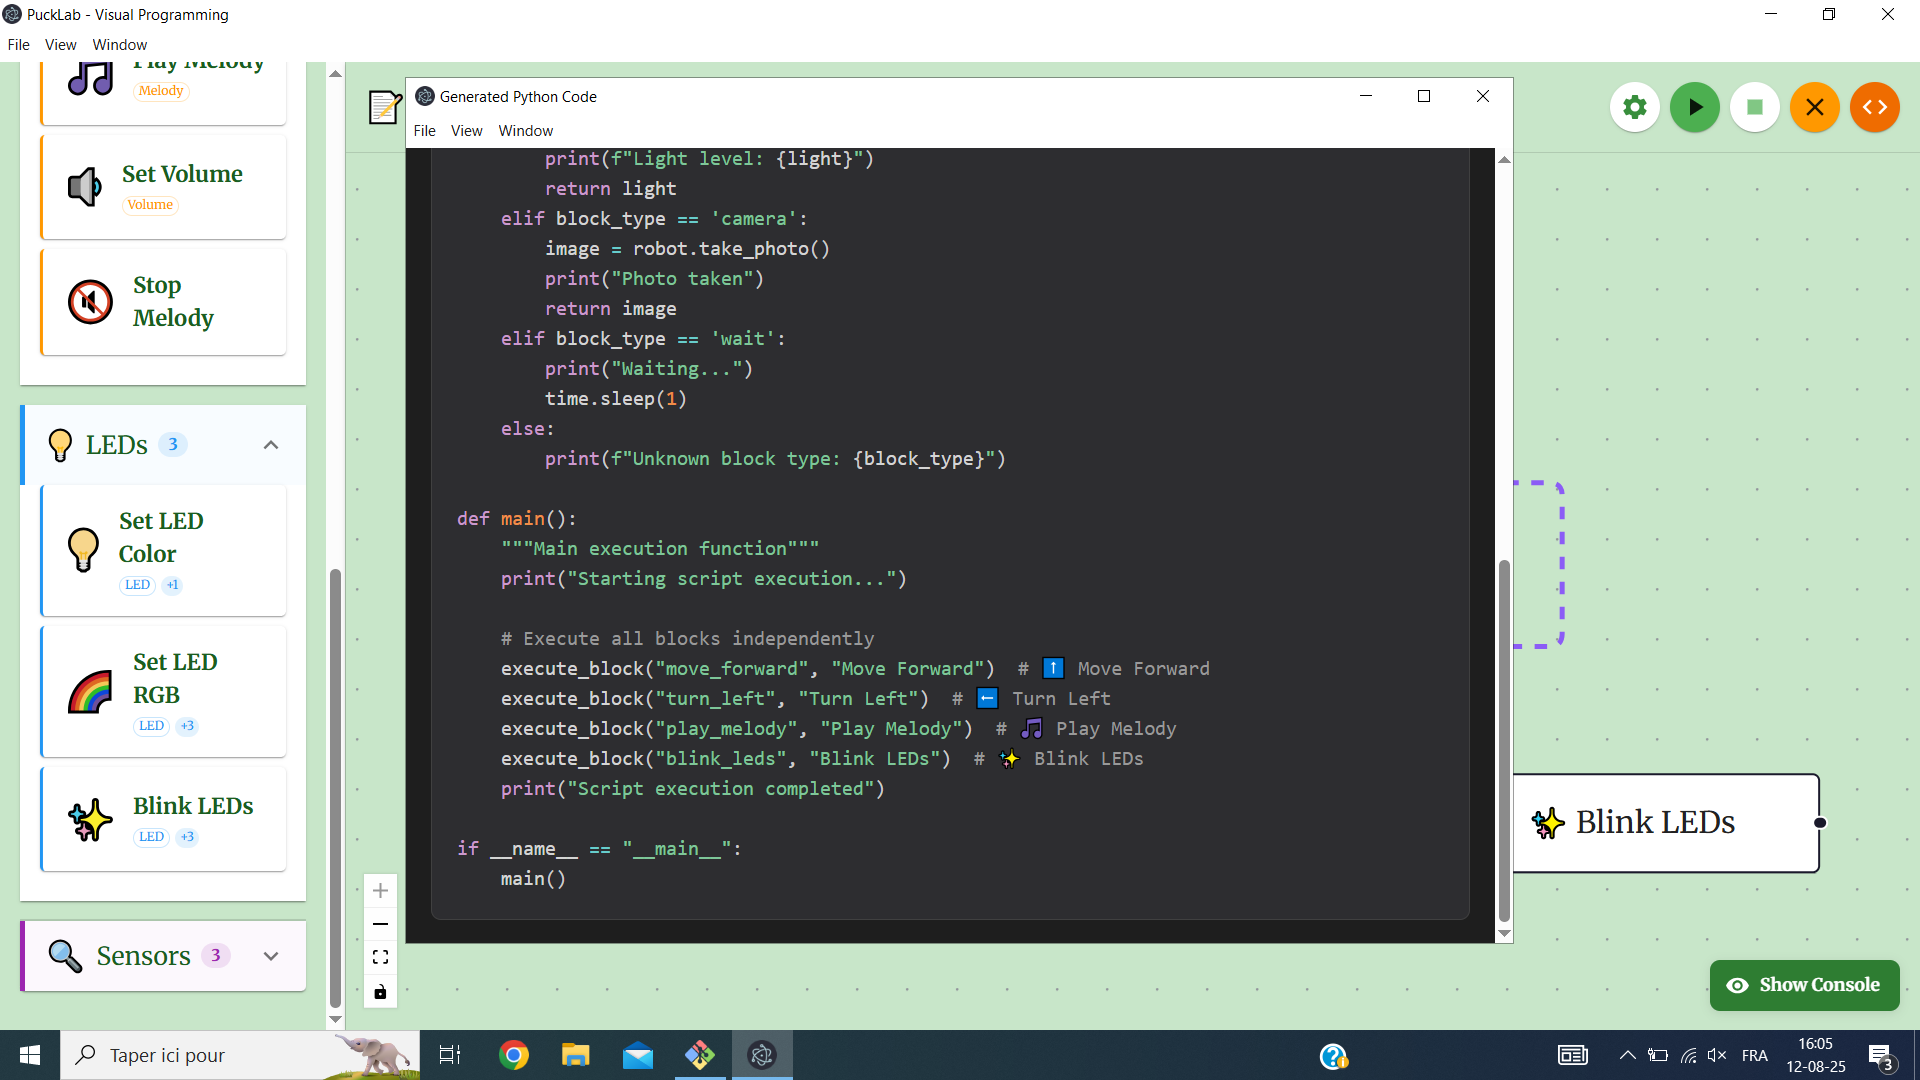
\includegraphics[width=\linewidth]{figures//screenshots//visual programming - age under 12 - code viewer opened.png}
        \caption{\label{fig:vp_ageunder12_codevieweropened} Écran - Programmation Visuelle (jeune - visualisateur de code ouvert)}
    \end{subfigure}

    \caption{\label{fig:screenshots-2} Captures d'écran de l'application Pucklab - 2}
\end{figure}

\begin{figure}[H]
    \centering

    \begin{subfigure}{0.45\linewidth}
        \centering
        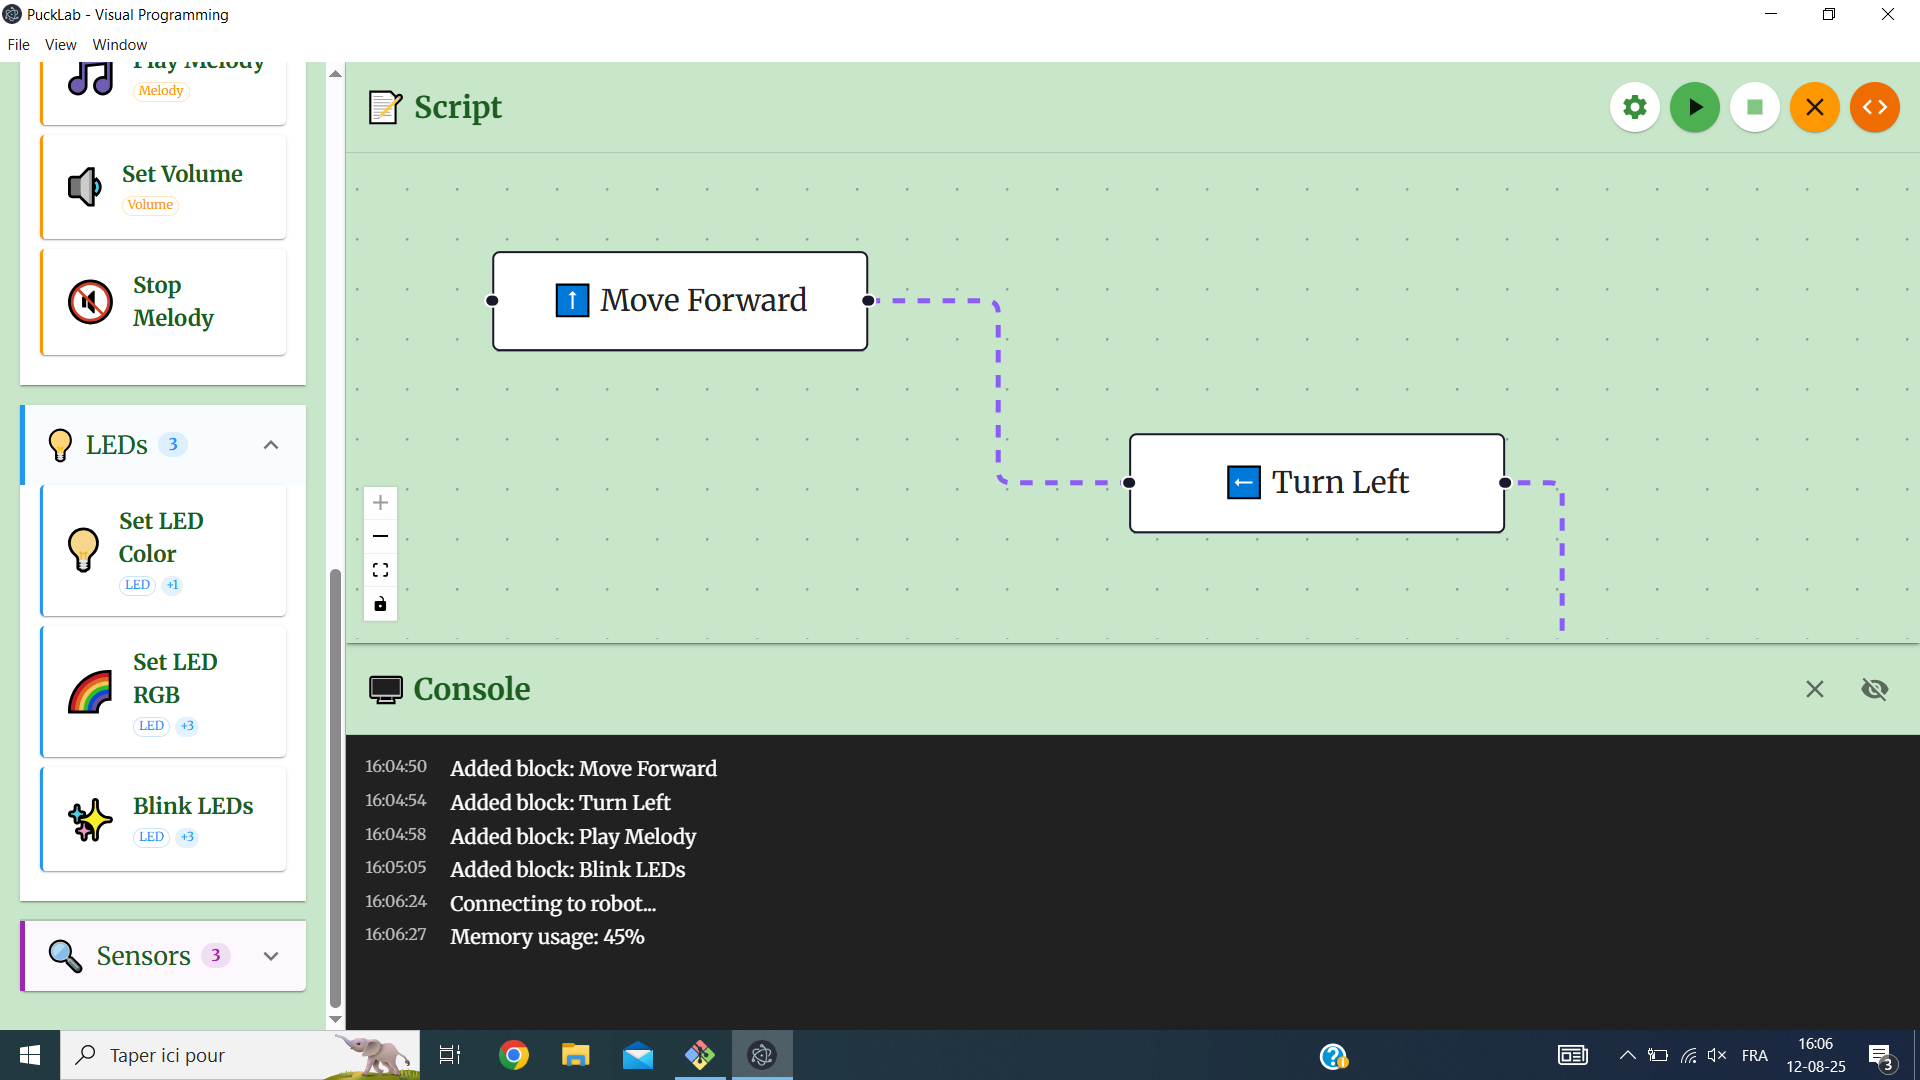
\includegraphics[width=\linewidth]{figures//screenshots//visual programming - age above 12.png}
        \caption{\label{fig:vp_ageabove12} Écran - Programmation Visuelle (adolescent)}
    \end{subfigure}
    \hfill
    \begin{subfigure}{0.45\linewidth}
        \centering
        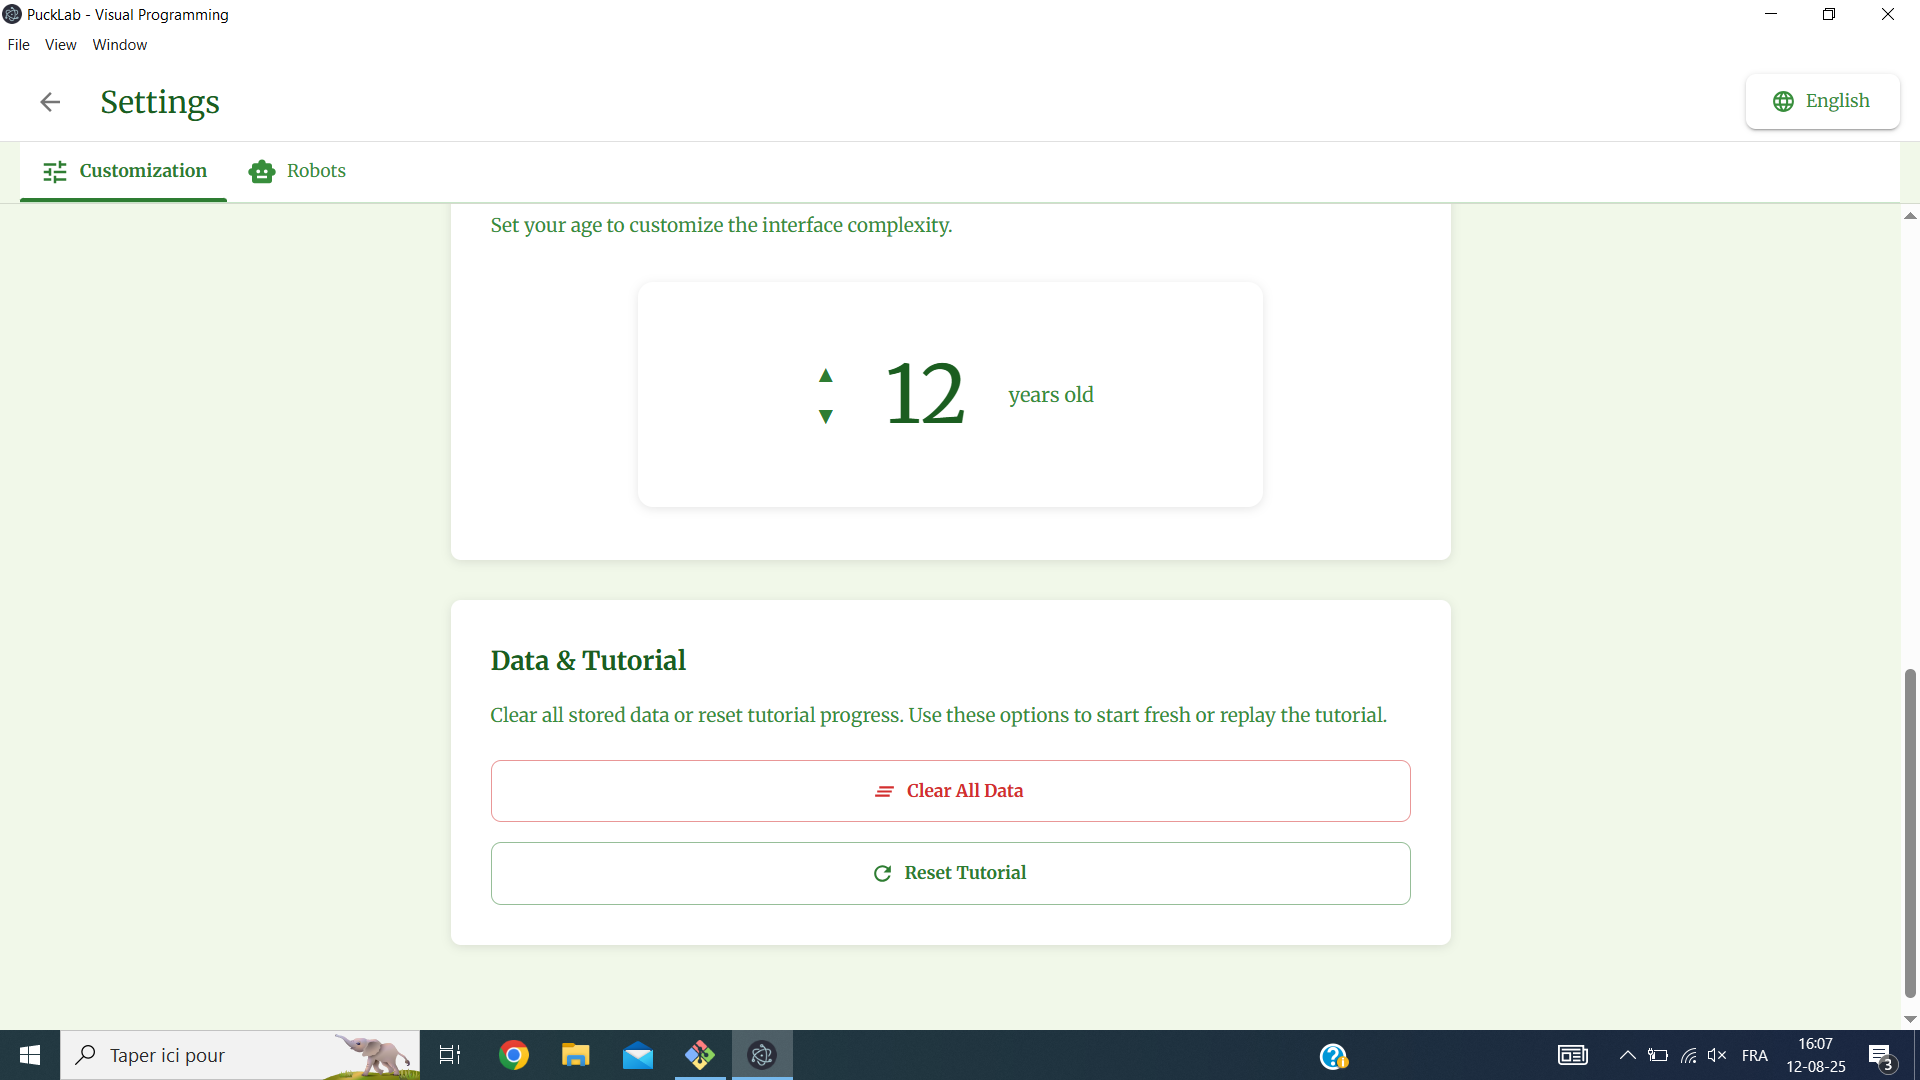
\includegraphics[width=\linewidth]{figures//screenshots//settings - customization tab.png}
        \caption{\label{fig:settings_customization} Écran - Paramètres de personnalisation}
    \end{subfigure}

    \vspace{0.25cm}

    \begin{subfigure}{0.45\linewidth}
        \centering
        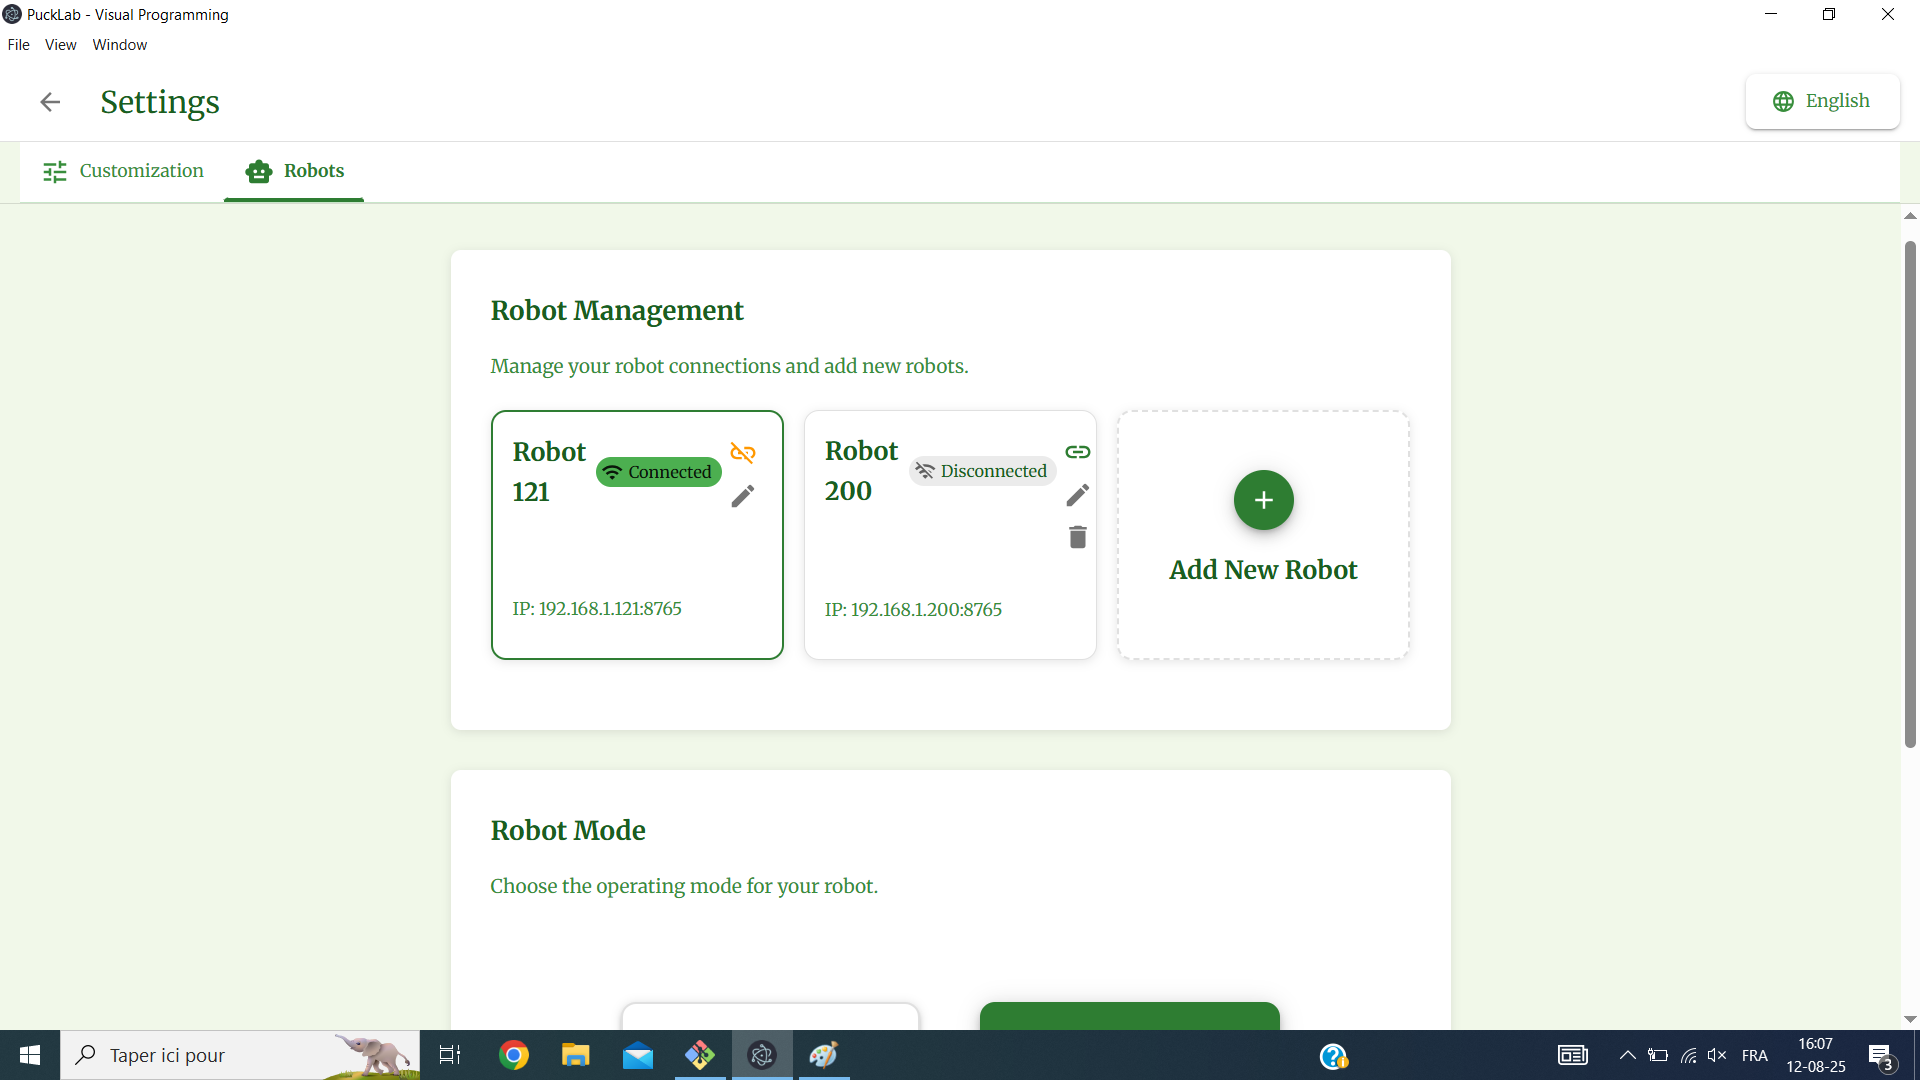
\includegraphics[width=\linewidth]{figures//screenshots//settings - robots tab.png}
        \caption{\label{fig:settings_robots} Écran - Paramètres sur les robots}
    \end{subfigure}

    \caption{\label{fig:screenshots-3} Captures d'écran de l'application Pucklab - 3}
\end{figure}

\subsection{Développement du firmware embarqué (robot)}

La seconde phase de développement a concerné le \textit{firmware}, conçu comme un serveur Python s’exécutant sur le Raspberry Pi du robot e-puck2. 
Ce serveur établit une communication bidirectionnelle via WebSocket avec l’interface Electron, exécute les commandes reçues, et transmet les états et données du robot en retour.

Là encore, une architecture en couches a été définie selon les principes de la \textit{clean architecture}, en séparant clairement les responsabilités entre la couche \textit{domaine}, la couche \textit{application}, et la couche \textit{infrastructure} en lien direct avec le matériel (moteurs, capteurs, LEDs, etc.).
